% Options for packages loaded elsewhere
\PassOptionsToPackage{unicode}{hyperref}
\PassOptionsToPackage{hyphens}{url}
%
\documentclass[
]{article}
\usepackage{lmodern}
\usepackage{amssymb,amsmath}
\usepackage{ifxetex,ifluatex}
\ifnum 0\ifxetex 1\fi\ifluatex 1\fi=0 % if pdftex
  \usepackage[T1]{fontenc}
  \usepackage[utf8]{inputenc}
  \usepackage{textcomp} % provide euro and other symbols
\else % if luatex or xetex
  \usepackage{unicode-math}
  \defaultfontfeatures{Scale=MatchLowercase}
  \defaultfontfeatures[\rmfamily]{Ligatures=TeX,Scale=1}
\fi
% Use upquote if available, for straight quotes in verbatim environments
\IfFileExists{upquote.sty}{\usepackage{upquote}}{}
\IfFileExists{microtype.sty}{% use microtype if available
  \usepackage[]{microtype}
  \UseMicrotypeSet[protrusion]{basicmath} % disable protrusion for tt fonts
}{}
\makeatletter
\@ifundefined{KOMAClassName}{% if non-KOMA class
  \IfFileExists{parskip.sty}{%
    \usepackage{parskip}
  }{% else
    \setlength{\parindent}{0pt}
    \setlength{\parskip}{6pt plus 2pt minus 1pt}}
}{% if KOMA class
  \KOMAoptions{parskip=half}}
\makeatother
\usepackage{xcolor}
\IfFileExists{xurl.sty}{\usepackage{xurl}}{} % add URL line breaks if available
\IfFileExists{bookmark.sty}{\usepackage{bookmark}}{\usepackage{hyperref}}
\hypersetup{
  pdftitle={CO\_sgs\_code\_forMS},
  hidelinks,
  pdfcreator={LaTeX via pandoc}}
\urlstyle{same} % disable monospaced font for URLs
\usepackage[margin=1in]{geometry}
\usepackage{color}
\usepackage{fancyvrb}
\newcommand{\VerbBar}{|}
\newcommand{\VERB}{\Verb[commandchars=\\\{\}]}
\DefineVerbatimEnvironment{Highlighting}{Verbatim}{commandchars=\\\{\}}
% Add ',fontsize=\small' for more characters per line
\usepackage{framed}
\definecolor{shadecolor}{RGB}{248,248,248}
\newenvironment{Shaded}{\begin{snugshade}}{\end{snugshade}}
\newcommand{\AlertTok}[1]{\textcolor[rgb]{0.94,0.16,0.16}{#1}}
\newcommand{\AnnotationTok}[1]{\textcolor[rgb]{0.56,0.35,0.01}{\textbf{\textit{#1}}}}
\newcommand{\AttributeTok}[1]{\textcolor[rgb]{0.77,0.63,0.00}{#1}}
\newcommand{\BaseNTok}[1]{\textcolor[rgb]{0.00,0.00,0.81}{#1}}
\newcommand{\BuiltInTok}[1]{#1}
\newcommand{\CharTok}[1]{\textcolor[rgb]{0.31,0.60,0.02}{#1}}
\newcommand{\CommentTok}[1]{\textcolor[rgb]{0.56,0.35,0.01}{\textit{#1}}}
\newcommand{\CommentVarTok}[1]{\textcolor[rgb]{0.56,0.35,0.01}{\textbf{\textit{#1}}}}
\newcommand{\ConstantTok}[1]{\textcolor[rgb]{0.00,0.00,0.00}{#1}}
\newcommand{\ControlFlowTok}[1]{\textcolor[rgb]{0.13,0.29,0.53}{\textbf{#1}}}
\newcommand{\DataTypeTok}[1]{\textcolor[rgb]{0.13,0.29,0.53}{#1}}
\newcommand{\DecValTok}[1]{\textcolor[rgb]{0.00,0.00,0.81}{#1}}
\newcommand{\DocumentationTok}[1]{\textcolor[rgb]{0.56,0.35,0.01}{\textbf{\textit{#1}}}}
\newcommand{\ErrorTok}[1]{\textcolor[rgb]{0.64,0.00,0.00}{\textbf{#1}}}
\newcommand{\ExtensionTok}[1]{#1}
\newcommand{\FloatTok}[1]{\textcolor[rgb]{0.00,0.00,0.81}{#1}}
\newcommand{\FunctionTok}[1]{\textcolor[rgb]{0.00,0.00,0.00}{#1}}
\newcommand{\ImportTok}[1]{#1}
\newcommand{\InformationTok}[1]{\textcolor[rgb]{0.56,0.35,0.01}{\textbf{\textit{#1}}}}
\newcommand{\KeywordTok}[1]{\textcolor[rgb]{0.13,0.29,0.53}{\textbf{#1}}}
\newcommand{\NormalTok}[1]{#1}
\newcommand{\OperatorTok}[1]{\textcolor[rgb]{0.81,0.36,0.00}{\textbf{#1}}}
\newcommand{\OtherTok}[1]{\textcolor[rgb]{0.56,0.35,0.01}{#1}}
\newcommand{\PreprocessorTok}[1]{\textcolor[rgb]{0.56,0.35,0.01}{\textit{#1}}}
\newcommand{\RegionMarkerTok}[1]{#1}
\newcommand{\SpecialCharTok}[1]{\textcolor[rgb]{0.00,0.00,0.00}{#1}}
\newcommand{\SpecialStringTok}[1]{\textcolor[rgb]{0.31,0.60,0.02}{#1}}
\newcommand{\StringTok}[1]{\textcolor[rgb]{0.31,0.60,0.02}{#1}}
\newcommand{\VariableTok}[1]{\textcolor[rgb]{0.00,0.00,0.00}{#1}}
\newcommand{\VerbatimStringTok}[1]{\textcolor[rgb]{0.31,0.60,0.02}{#1}}
\newcommand{\WarningTok}[1]{\textcolor[rgb]{0.56,0.35,0.01}{\textbf{\textit{#1}}}}
\usepackage{graphicx}
\makeatletter
\def\maxwidth{\ifdim\Gin@nat@width>\linewidth\linewidth\else\Gin@nat@width\fi}
\def\maxheight{\ifdim\Gin@nat@height>\textheight\textheight\else\Gin@nat@height\fi}
\makeatother
% Scale images if necessary, so that they will not overflow the page
% margins by default, and it is still possible to overwrite the defaults
% using explicit options in \includegraphics[width, height, ...]{}
\setkeys{Gin}{width=\maxwidth,height=\maxheight,keepaspectratio}
% Set default figure placement to htbp
\makeatletter
\def\fps@figure{htbp}
\makeatother
\setlength{\emergencystretch}{3em} % prevent overfull lines
\providecommand{\tightlist}{%
  \setlength{\itemsep}{0pt}\setlength{\parskip}{0pt}}
\setcounter{secnumdepth}{-\maxdimen} % remove section numbering
\ifluatex
  \usepackage{selnolig}  % disable illegal ligatures
\fi

\title{CO\_sgs\_code\_forMS}
\author{}
\date{\vspace{-2.5em}}

\begin{document}
\maketitle

Load packages

\begin{Shaded}
\begin{Highlighting}[]
\KeywordTok{require}\NormalTok{(effects)}
\KeywordTok{require}\NormalTok{(lattice)}
\KeywordTok{require}\NormalTok{(latticeExtra)}
\KeywordTok{require}\NormalTok{(gridExtra)}
\KeywordTok{require}\NormalTok{(grid)}
\KeywordTok{require}\NormalTok{(ggpubr)}
\KeywordTok{require}\NormalTok{(lme4)}
\KeywordTok{require}\NormalTok{(ggeffects)}
\KeywordTok{require}\NormalTok{(tidyverse)}
\end{Highlighting}
\end{Shaded}

Load model output data

\begin{Shaded}
\begin{Highlighting}[]
\CommentTok{\#\#\#\# set wd \#\#\#\#}
\KeywordTok{setwd}\NormalTok{(}\StringTok{"/Users/Alice/Dropbox/Grad School/Research/Trait Project/CO\_sgs Analysis"}\NormalTok{)}
\CommentTok{\#get model result data into the environment}
\KeywordTok{load}\NormalTok{(}\StringTok{"./SCRIPTS/models\_11232020.RData"}\NormalTok{) }\CommentTok{\#change the file name to the most current version of model runs}
\end{Highlighting}
\end{Shaded}

Make a figure of model results for LDMC, RDMC, and TLP for forb and gram
survival

\begin{Shaded}
\begin{Highlighting}[]
\CommentTok{\#make figure for graminoid survival}

\CommentTok{\#get 2.5 and 97.5 percentiles of the distribution}
\NormalTok{meanSPEI\_G \textless{}{-}}\StringTok{ }\KeywordTok{mean}\NormalTok{(CO\_grams}\OperatorTok{$}\NormalTok{SPEI\_s)}
\NormalTok{sdSPEI\_G \textless{}{-}}\StringTok{ }\KeywordTok{sd}\NormalTok{(CO\_grams}\OperatorTok{$}\NormalTok{SPEI\_s)}
\CommentTok{\#get 97.5 quantile of the distribution}
\NormalTok{SPEI\_}\DecValTok{97}\NormalTok{\_}\DecValTok{5}\NormalTok{\_G \textless{}{-}}\StringTok{ }\KeywordTok{qnorm}\NormalTok{(.}\DecValTok{975}\NormalTok{, meanSPEI\_G, sdSPEI\_G) }
\NormalTok{SPEI\_}\DecValTok{2}\NormalTok{\_}\DecValTok{5}\NormalTok{\_G \textless{}{-}}\StringTok{ }\KeywordTok{qnorm}\NormalTok{(.}\DecValTok{025}\NormalTok{, meanSPEI\_G, sdSPEI\_G)}

\NormalTok{spei\_vals \textless{}{-}}\StringTok{ }\KeywordTok{c}\NormalTok{(SPEI\_}\DecValTok{2}\NormalTok{\_}\DecValTok{5}\NormalTok{\_G, SPEI\_}\DecValTok{97}\NormalTok{\_}\DecValTok{5}\NormalTok{\_G)}

\CommentTok{\#for TLP\_s}
\NormalTok{TLP\_vals \textless{}{-}}\StringTok{ }\KeywordTok{seq}\NormalTok{(}\KeywordTok{min}\NormalTok{(CO\_grams}\OperatorTok{$}\NormalTok{TLP\_s, }\DataTypeTok{na.rm =} \OtherTok{TRUE}\NormalTok{), }\KeywordTok{max}\NormalTok{(CO\_grams}\OperatorTok{$}\NormalTok{TLP\_s, }\DataTypeTok{na.rm =} \OtherTok{TRUE}\NormalTok{), }\DataTypeTok{length.out =} \DecValTok{20}\NormalTok{)}
\NormalTok{TLP\_G\_dat \textless{}{-}}\StringTok{ }\KeywordTok{ggpredict}\NormalTok{(m1\_grams, }\DataTypeTok{terms =} \KeywordTok{c}\NormalTok{(}\StringTok{"TLP\_s[TLP\_vals]"}\NormalTok{, }\StringTok{"SPEI\_s[spei\_vals]"}\NormalTok{), }\DataTypeTok{type =} \StringTok{"fixed"}\NormalTok{, }\DataTypeTok{back.transform =} \OtherTok{TRUE}\NormalTok{)}


\CommentTok{\#for LDMC\_s}
\NormalTok{LDMC\_vals \textless{}{-}}\StringTok{ }\KeywordTok{seq}\NormalTok{(}\KeywordTok{min}\NormalTok{(CO\_grams}\OperatorTok{$}\NormalTok{LDMC\_s, }\DataTypeTok{na.rm =} \OtherTok{TRUE}\NormalTok{), }\KeywordTok{max}\NormalTok{(CO\_grams}\OperatorTok{$}\NormalTok{LDMC\_s, }\DataTypeTok{na.rm =} \OtherTok{TRUE}\NormalTok{), }\DataTypeTok{length.out =} \DecValTok{20}\NormalTok{)}
\NormalTok{LDMC\_G\_dat \textless{}{-}}\StringTok{ }\KeywordTok{ggpredict}\NormalTok{(m2\_grams, }\DataTypeTok{terms =} \KeywordTok{c}\NormalTok{(}\StringTok{"LDMC\_s[LDMC\_vals]"}\NormalTok{, }\StringTok{"SPEI\_s[spei\_vals]"}\NormalTok{), }\DataTypeTok{type =} \StringTok{"fixed"}\NormalTok{, }\DataTypeTok{back.transform =} \OtherTok{TRUE}\NormalTok{)}

\CommentTok{\#for RDMC\_s}
\NormalTok{RDMC\_vals \textless{}{-}}\StringTok{ }\KeywordTok{seq}\NormalTok{(}\KeywordTok{min}\NormalTok{(CO\_grams}\OperatorTok{$}\NormalTok{RDMC\_s, }\DataTypeTok{na.rm =} \OtherTok{TRUE}\NormalTok{), }\KeywordTok{max}\NormalTok{(CO\_grams}\OperatorTok{$}\NormalTok{RDMC\_s, }\DataTypeTok{na.rm =} \OtherTok{TRUE}\NormalTok{), }\DataTypeTok{length.out =} \DecValTok{20}\NormalTok{)}
\NormalTok{RDMC\_G\_dat \textless{}{-}}\StringTok{ }\KeywordTok{ggpredict}\NormalTok{(m9, }\DataTypeTok{terms =} \KeywordTok{c}\NormalTok{(}\StringTok{"RDMC\_s[RDMC\_vals]"}\NormalTok{, }\StringTok{"SPEI\_s[spei\_vals]"}\NormalTok{), }\DataTypeTok{type =} \StringTok{"fixed"}\NormalTok{, }\DataTypeTok{back.transform =} \OtherTok{TRUE}\NormalTok{)}


\CommentTok{\#make a data.frame to contain all of the values for each trait}
\NormalTok{GramDat \textless{}{-}}\StringTok{ }\KeywordTok{data.frame}\NormalTok{(}\DataTypeTok{trait =} \KeywordTok{c}\NormalTok{(}\StringTok{"scaled(Turgor Loss Point) (MPa)"}\NormalTok{), }\DataTypeTok{x =}\NormalTok{ TLP\_G\_dat}\OperatorTok{$}\NormalTok{x, }\DataTypeTok{GramSurv =}\NormalTok{ TLP\_G\_dat}\OperatorTok{$}\NormalTok{predicted, }\DataTypeTok{CI\_low =}\NormalTok{ TLP\_G\_dat}\OperatorTok{$}\NormalTok{conf.low, }\DataTypeTok{CI\_high =}\NormalTok{ TLP\_G\_dat}\OperatorTok{$}\NormalTok{conf.high, }\DataTypeTok{SPEI =}\NormalTok{ TLP\_G\_dat}\OperatorTok{$}\NormalTok{group, }\DataTypeTok{lab =} \StringTok{"A"}\NormalTok{)}

\NormalTok{GramDat \textless{}{-}}\StringTok{ }\KeywordTok{rbind}\NormalTok{(GramDat, }\KeywordTok{data.frame}\NormalTok{(}\DataTypeTok{trait =} \KeywordTok{c}\NormalTok{(}\StringTok{"scaled(Leaf Dry Matter Content) (g/g)"}\NormalTok{), }\DataTypeTok{x =}\NormalTok{ LDMC\_G\_dat}\OperatorTok{$}\NormalTok{x, }\DataTypeTok{GramSurv =}\NormalTok{ LDMC\_G\_dat}\OperatorTok{$}\NormalTok{predicted, }\DataTypeTok{CI\_low =}\NormalTok{ LDMC\_G\_dat}\OperatorTok{$}\NormalTok{conf.low, }\DataTypeTok{CI\_high =}\NormalTok{ LDMC\_G\_dat}\OperatorTok{$}\NormalTok{conf.high, }\DataTypeTok{SPEI =}\NormalTok{ LDMC\_G\_dat}\OperatorTok{$}\NormalTok{group, }\DataTypeTok{lab =} \StringTok{"B"}\NormalTok{))}

\NormalTok{GramDat \textless{}{-}}\StringTok{ }\KeywordTok{rbind}\NormalTok{(GramDat, }\KeywordTok{data.frame}\NormalTok{(}\DataTypeTok{trait =} \KeywordTok{c}\NormalTok{(}\StringTok{"scaled(Root Dry Matter Content) (g/g)"}\NormalTok{), }\DataTypeTok{x =}\NormalTok{ RDMC\_G\_dat}\OperatorTok{$}\NormalTok{x, }\DataTypeTok{GramSurv =}\NormalTok{ RDMC\_G\_dat}\OperatorTok{$}\NormalTok{predicted, }\DataTypeTok{CI\_low =}\NormalTok{ RDMC\_G\_dat}\OperatorTok{$}\NormalTok{conf.low, }\DataTypeTok{CI\_high =}\NormalTok{ RDMC\_G\_dat}\OperatorTok{$}\NormalTok{conf.high, }\DataTypeTok{SPEI =}\NormalTok{ RDMC\_G\_dat}\OperatorTok{$}\NormalTok{group, }\DataTypeTok{lab =} \StringTok{"C"}\NormalTok{))}

\CommentTok{\#make data for rug plot}
\NormalTok{RugDat\_G \textless{}{-}}\StringTok{  }\KeywordTok{data.frame}\NormalTok{(}\DataTypeTok{rug =}\NormalTok{ CO\_grams}\OperatorTok{$}\NormalTok{TLP\_s, }\DataTypeTok{trait =} \StringTok{"scaled(Turgor Loss Point) (MPa)"}\NormalTok{)}
\NormalTok{RugDat\_G \textless{}{-}}\StringTok{ }\KeywordTok{rbind}\NormalTok{(RugDat\_G, }\KeywordTok{data.frame}\NormalTok{(}\DataTypeTok{rug =}\NormalTok{ CO\_grams}\OperatorTok{$}\NormalTok{LDMC\_s, }\DataTypeTok{trait =} \StringTok{"scaled(Leaf Dry Matter Content) (g/g)"}\NormalTok{))}
\NormalTok{RugDat\_G \textless{}{-}}\StringTok{ }\KeywordTok{rbind}\NormalTok{(RugDat\_G, }\KeywordTok{data.frame}\NormalTok{(}\DataTypeTok{rug =}\NormalTok{ CO\_grams}\OperatorTok{$}\NormalTok{RDMC\_s, }\DataTypeTok{trait =} \StringTok{"scaled(Root Dry Matter Content) (g/g)"}\NormalTok{))}

\CommentTok{\#text for labels}
\NormalTok{dat\_text \textless{}{-}}\StringTok{ }\KeywordTok{data.frame}\NormalTok{(}
  \DataTypeTok{label =} \KeywordTok{c}\NormalTok{(}\StringTok{"D"}\NormalTok{, }\StringTok{"E"}\NormalTok{, }\StringTok{"F"}\NormalTok{),}
  \DataTypeTok{trait =} \KeywordTok{c}\NormalTok{(}\StringTok{"scaled(Turgor Loss Point) (MPa)"}\NormalTok{, }\StringTok{"scaled(Leaf Dry Matter Content) (g/g)"}\NormalTok{, }\StringTok{"scaled(Root Dry Matter Content) (g/g)"}\NormalTok{),}
  \DataTypeTok{x    =} \KeywordTok{c}\NormalTok{(}\KeywordTok{min}\NormalTok{(TLP\_G\_dat}\OperatorTok{$}\NormalTok{x),}\KeywordTok{min}\NormalTok{(LDMC\_G\_dat}\OperatorTok{$}\NormalTok{x),}\KeywordTok{min}\NormalTok{(RDMC\_G\_dat}\OperatorTok{$}\NormalTok{x)),}
  \DataTypeTok{y     =} \KeywordTok{c}\NormalTok{(}\DecValTok{1}\NormalTok{,}\DecValTok{1}\NormalTok{,}\DecValTok{1}\NormalTok{)}
\NormalTok{)}

\CommentTok{\#make a multipanel figure that shows only the graminoid survival probs for 3 traits}
\NormalTok{gramSurvFigure \textless{}{-}}\StringTok{ }\KeywordTok{ggplot}\NormalTok{(}\DataTypeTok{data =}\NormalTok{ GramDat) }\OperatorTok{+}
\StringTok{  }\KeywordTok{geom\_ribbon}\NormalTok{(}\KeywordTok{aes}\NormalTok{(}\DataTypeTok{x =}\NormalTok{ x, }\DataTypeTok{ymin =}\NormalTok{ CI\_low, }\DataTypeTok{ymax =}\NormalTok{ CI\_high, }\DataTypeTok{fill =}\NormalTok{ SPEI), }\DataTypeTok{alpha =} \FloatTok{0.3}\NormalTok{) }\OperatorTok{+}
\StringTok{  }\KeywordTok{geom\_line}\NormalTok{(}\KeywordTok{aes}\NormalTok{(}\DataTypeTok{x=}\NormalTok{x, GramSurv, }\DataTypeTok{col =}\NormalTok{ SPEI))  }\OperatorTok{+}\StringTok{ }
\StringTok{  }\KeywordTok{geom\_rug}\NormalTok{(}\KeywordTok{aes}\NormalTok{(}\DataTypeTok{x =}\NormalTok{ rug), }\DataTypeTok{data =}\NormalTok{ RugDat\_G) }\OperatorTok{+}
\StringTok{  }\KeywordTok{ggtitle}\NormalTok{(}\StringTok{"Observations"}\NormalTok{) }\OperatorTok{+}
\StringTok{  }\KeywordTok{xlab}\NormalTok{(}\OtherTok{NULL}\NormalTok{) }\OperatorTok{+}
\StringTok{  }\KeywordTok{ylab}\NormalTok{(}\StringTok{"P(Graminoid Survival)"}\NormalTok{) }\OperatorTok{+}
\StringTok{  }\KeywordTok{scale\_y\_continuous}\NormalTok{(}\DataTypeTok{limits =} \KeywordTok{c}\NormalTok{(}\DecValTok{0}\NormalTok{,}\DecValTok{1}\NormalTok{)) }\OperatorTok{+}
\StringTok{  }\KeywordTok{scale\_color\_manual}\NormalTok{(}\DataTypeTok{labels =} \KeywordTok{c}\NormalTok{(}\StringTok{"dry year"}\NormalTok{, }\StringTok{"wet year"}\NormalTok{), }\DataTypeTok{values =} \KeywordTok{c}\NormalTok{(}\StringTok{"goldenrod1"}\NormalTok{, }\StringTok{"royalblue2"}\NormalTok{), }\DataTypeTok{guide =} \OtherTok{FALSE}\NormalTok{) }\OperatorTok{+}
\StringTok{  }\KeywordTok{scale\_fill\_manual}\NormalTok{(}\DataTypeTok{values =} \KeywordTok{c}\NormalTok{(}\StringTok{"goldenrod1"}\NormalTok{, }\StringTok{"royalblue2"}\NormalTok{), }\DataTypeTok{guide =} \OtherTok{FALSE}\NormalTok{) }\OperatorTok{+}
\StringTok{  }\KeywordTok{facet\_wrap}\NormalTok{(}\KeywordTok{vars}\NormalTok{(trait), }\DataTypeTok{scales =} \StringTok{"free\_x"}\NormalTok{, }\DataTypeTok{strip.position =}  \StringTok{"bottom"}\NormalTok{) }\OperatorTok{+}
\StringTok{  }\KeywordTok{theme\_classic}\NormalTok{()}\OperatorTok{+}
\StringTok{  }\KeywordTok{theme}\NormalTok{(}\DataTypeTok{legend.position =} \StringTok{"bottom"}\NormalTok{, }\DataTypeTok{legend.title =} \KeywordTok{element\_blank}\NormalTok{(), }\DataTypeTok{legend.background =} \KeywordTok{element\_rect}\NormalTok{(}\DataTypeTok{fill=}\StringTok{"grey95"}\NormalTok{,}\DataTypeTok{size=}\FloatTok{0.5}\NormalTok{, }\DataTypeTok{linetype=}\StringTok{"solid"}\NormalTok{), }\DataTypeTok{strip.background =} \KeywordTok{element\_rect}\NormalTok{(}\DataTypeTok{colour=}\OtherTok{NA}\NormalTok{, }\DataTypeTok{fill=}\OtherTok{NA}\NormalTok{), }\DataTypeTok{strip.placement =} \StringTok{"outside"}\NormalTok{, }\DataTypeTok{strip.text.x =} \KeywordTok{element\_text}\NormalTok{(}\DataTypeTok{margin =} \KeywordTok{margin}\NormalTok{(}\DecValTok{0}\NormalTok{, }\DecValTok{0}\NormalTok{, }\FloatTok{1.5}\NormalTok{, }\DecValTok{0}\NormalTok{)), }\DataTypeTok{plot.title =} \KeywordTok{element\_text}\NormalTok{(}\DataTypeTok{hjust =} \FloatTok{0.5}\NormalTok{, }\DataTypeTok{size =} \DecValTok{13}\NormalTok{, }\DataTypeTok{face =} \StringTok{"bold"}\NormalTok{)) }\OperatorTok{+}
\StringTok{  }\KeywordTok{geom\_text}\NormalTok{(}\DataTypeTok{data=}\NormalTok{ dat\_text, }\DataTypeTok{mapping =} \KeywordTok{aes}\NormalTok{(}\DataTypeTok{x =}\NormalTok{ x, }\DataTypeTok{y =}\NormalTok{ y, }\DataTypeTok{label =}\NormalTok{ label), }\DataTypeTok{size =} \DecValTok{3}\NormalTok{, }\DataTypeTok{fontface =} \StringTok{"bold"}\NormalTok{)}
\end{Highlighting}
\end{Shaded}

make figure for forb survival

\begin{Shaded}
\begin{Highlighting}[]
\CommentTok{\#get 2.5 and 97.5 percentiles of the distribution}
\NormalTok{meanSPEI\_F \textless{}{-}}\StringTok{ }\KeywordTok{mean}\NormalTok{(CO\_point\_all}\OperatorTok{$}\NormalTok{SPEI\_s)}
\NormalTok{sdSPEI\_F \textless{}{-}}\StringTok{ }\KeywordTok{sd}\NormalTok{(CO\_point\_all}\OperatorTok{$}\NormalTok{SPEI\_s)}
\CommentTok{\#get 97.5 quantile of the distribution}
\NormalTok{SPEI\_}\DecValTok{97}\NormalTok{\_}\DecValTok{5}\NormalTok{\_F \textless{}{-}}\StringTok{ }\KeywordTok{qnorm}\NormalTok{(.}\DecValTok{975}\NormalTok{, meanSPEI\_F, sdSPEI\_F) }
\NormalTok{SPEI\_}\DecValTok{2}\NormalTok{\_}\DecValTok{5}\NormalTok{\_G \textless{}{-}}\StringTok{ }\KeywordTok{qnorm}\NormalTok{(.}\DecValTok{025}\NormalTok{, meanSPEI\_F, sdSPEI\_F)}

\NormalTok{spei\_vals \textless{}{-}}\StringTok{ }\KeywordTok{c}\NormalTok{(SPEI\_}\DecValTok{2}\NormalTok{\_}\DecValTok{5}\NormalTok{\_G, SPEI\_}\DecValTok{97}\NormalTok{\_}\DecValTok{5}\NormalTok{\_G)}

\CommentTok{\#for TLP\_s}
\NormalTok{TLP\_vals \textless{}{-}}\StringTok{ }\KeywordTok{seq}\NormalTok{(}\KeywordTok{min}\NormalTok{(CO\_point\_all}\OperatorTok{$}\NormalTok{TLP\_s, }\DataTypeTok{na.rm =} \OtherTok{TRUE}\NormalTok{), }\KeywordTok{max}\NormalTok{(CO\_point\_all}\OperatorTok{$}\NormalTok{TLP\_s, }\DataTypeTok{na.rm =} \OtherTok{TRUE}\NormalTok{), }\DataTypeTok{length.out =} \DecValTok{20}\NormalTok{)}
\NormalTok{TLP\_F\_dat \textless{}{-}}\StringTok{ }\KeywordTok{ggpredict}\NormalTok{(m3, }\DataTypeTok{terms =} \KeywordTok{c}\NormalTok{(}\StringTok{"TLP\_s[TLP\_vals]"}\NormalTok{, }\StringTok{"SPEI\_s[spei\_vals]"}\NormalTok{), }\DataTypeTok{type =} \StringTok{"fixed"}\NormalTok{, }\DataTypeTok{back.transform =} \OtherTok{TRUE}\NormalTok{)}


\CommentTok{\#for LDMC\_s}
\NormalTok{LDMC\_vals \textless{}{-}}\StringTok{ }\KeywordTok{seq}\NormalTok{(}\KeywordTok{min}\NormalTok{(CO\_point\_all}\OperatorTok{$}\NormalTok{LDMC\_s, }\DataTypeTok{na.rm =} \OtherTok{TRUE}\NormalTok{), }\KeywordTok{max}\NormalTok{(CO\_point\_all}\OperatorTok{$}\NormalTok{LDMC\_s, }\DataTypeTok{na.rm =} \OtherTok{TRUE}\NormalTok{), }\DataTypeTok{length.out =} \DecValTok{20}\NormalTok{)}
\NormalTok{LDMC\_F\_dat \textless{}{-}}\StringTok{ }\KeywordTok{ggpredict}\NormalTok{(m4, }\DataTypeTok{terms =} \KeywordTok{c}\NormalTok{(}\StringTok{"LDMC\_s[LDMC\_vals]"}\NormalTok{, }\StringTok{"SPEI\_s[spei\_vals]"}\NormalTok{), }\DataTypeTok{type =} \StringTok{"fixed"}\NormalTok{, }\DataTypeTok{back.transform =} \OtherTok{TRUE}\NormalTok{)}

\CommentTok{\#for RDMC\_s}
\NormalTok{RDMC\_vals \textless{}{-}}\StringTok{ }\KeywordTok{seq}\NormalTok{(}\KeywordTok{min}\NormalTok{(CO\_point\_all}\OperatorTok{$}\NormalTok{RDMC\_s, }\DataTypeTok{na.rm =} \OtherTok{TRUE}\NormalTok{), }\KeywordTok{max}\NormalTok{(CO\_point\_all}\OperatorTok{$}\NormalTok{RDMC\_s, }\DataTypeTok{na.rm =} \OtherTok{TRUE}\NormalTok{), }\DataTypeTok{length.out =} \DecValTok{20}\NormalTok{)}
\NormalTok{RDMC\_F\_dat \textless{}{-}}\StringTok{ }\KeywordTok{ggpredict}\NormalTok{(m11, }\DataTypeTok{terms =} \KeywordTok{c}\NormalTok{(}\StringTok{"RDMC\_s[RDMC\_vals]"}\NormalTok{, }\StringTok{"SPEI\_s[spei\_vals]"}\NormalTok{), }\DataTypeTok{type =} \StringTok{"fixed"}\NormalTok{, }\DataTypeTok{back.transform =} \OtherTok{TRUE}\NormalTok{)}


\CommentTok{\#make a data.frame to contain all of the values for each trait}
\NormalTok{ForbDat \textless{}{-}}\StringTok{ }\KeywordTok{data.frame}\NormalTok{(}\DataTypeTok{trait =} \KeywordTok{c}\NormalTok{(}\StringTok{"scaled(Turgor Loss Point) (MPa)"}\NormalTok{), }\DataTypeTok{x =}\NormalTok{ TLP\_F\_dat}\OperatorTok{$}\NormalTok{x, }\DataTypeTok{ForbSurv =}\NormalTok{ TLP\_F\_dat}\OperatorTok{$}\NormalTok{predicted, }\DataTypeTok{CI\_low =}\NormalTok{ TLP\_F\_dat}\OperatorTok{$}\NormalTok{conf.low, }\DataTypeTok{CI\_high =}\NormalTok{ TLP\_F\_dat}\OperatorTok{$}\NormalTok{conf.high, }\DataTypeTok{SPEI =}\NormalTok{ TLP\_F\_dat}\OperatorTok{$}\NormalTok{group, }\DataTypeTok{lab =} \StringTok{"G"}\NormalTok{)}

\NormalTok{ForbDat \textless{}{-}}\StringTok{ }\KeywordTok{rbind}\NormalTok{(ForbDat, }\KeywordTok{data.frame}\NormalTok{(}\DataTypeTok{trait =} \KeywordTok{c}\NormalTok{(}\StringTok{"scaled(Leaf Dry Matter Content) (g/g)"}\NormalTok{), }\DataTypeTok{x =}\NormalTok{ LDMC\_F\_dat}\OperatorTok{$}\NormalTok{x, }\DataTypeTok{ForbSurv =}\NormalTok{ LDMC\_F\_dat}\OperatorTok{$}\NormalTok{predicted, }\DataTypeTok{CI\_low =}\NormalTok{ LDMC\_F\_dat}\OperatorTok{$}\NormalTok{conf.low, }\DataTypeTok{CI\_high =}\NormalTok{ LDMC\_F\_dat}\OperatorTok{$}\NormalTok{conf.high, }\DataTypeTok{SPEI =}\NormalTok{ LDMC\_F\_dat}\OperatorTok{$}\NormalTok{group, }\DataTypeTok{lab =} \StringTok{"H"}\NormalTok{))}

\NormalTok{ForbDat \textless{}{-}}\StringTok{ }\KeywordTok{rbind}\NormalTok{(ForbDat, }\KeywordTok{data.frame}\NormalTok{(}\DataTypeTok{trait =} \KeywordTok{c}\NormalTok{(}\StringTok{"scaled(Root Dry Matter Content) (g/g)"}\NormalTok{), }\DataTypeTok{x =}\NormalTok{ RDMC\_F\_dat}\OperatorTok{$}\NormalTok{x, }\DataTypeTok{ForbSurv =}\NormalTok{ RDMC\_F\_dat}\OperatorTok{$}\NormalTok{predicted, }\DataTypeTok{CI\_low =}\NormalTok{ RDMC\_F\_dat}\OperatorTok{$}\NormalTok{conf.low, }\DataTypeTok{CI\_high =}\NormalTok{ RDMC\_F\_dat}\OperatorTok{$}\NormalTok{conf.high, }\DataTypeTok{SPEI =}\NormalTok{ RDMC\_F\_dat}\OperatorTok{$}\NormalTok{group, }\DataTypeTok{lab =} \StringTok{"I"}\NormalTok{))}

\CommentTok{\#make data for rug plot}
\NormalTok{RugDat\_F \textless{}{-}}\StringTok{  }\KeywordTok{data.frame}\NormalTok{(}\DataTypeTok{rug =}\NormalTok{ CO\_point\_all}\OperatorTok{$}\NormalTok{TLP\_s, }\DataTypeTok{trait =} \StringTok{"scaled(Turgor Loss Point) (MPa)"}\NormalTok{)}
\NormalTok{RugDat\_F \textless{}{-}}\StringTok{ }\KeywordTok{rbind}\NormalTok{(RugDat\_F, }\KeywordTok{data.frame}\NormalTok{(}\DataTypeTok{rug =}\NormalTok{ CO\_point\_all}\OperatorTok{$}\NormalTok{LDMC\_s, }\DataTypeTok{trait =} \StringTok{"scaled(Leaf Dry Matter Content) (g/g)"}\NormalTok{))}
\NormalTok{RugDat\_F \textless{}{-}}\StringTok{ }\KeywordTok{rbind}\NormalTok{(RugDat\_F, }\KeywordTok{data.frame}\NormalTok{(}\DataTypeTok{rug =}\NormalTok{ CO\_point\_all}\OperatorTok{$}\NormalTok{RDMC\_s, }\DataTypeTok{trait =} \StringTok{"scaled(Root Dry Matter Content) (g/g)"}\NormalTok{))}

\CommentTok{\#text for labels}
\NormalTok{dat\_text \textless{}{-}}\StringTok{ }\KeywordTok{data.frame}\NormalTok{(}
  \DataTypeTok{label =} \KeywordTok{c}\NormalTok{(}\StringTok{"G"}\NormalTok{, }\StringTok{"H"}\NormalTok{, }\StringTok{"I"}\NormalTok{),}
  \DataTypeTok{trait =} \KeywordTok{c}\NormalTok{(}\StringTok{"scaled(Turgor Loss Point) (MPa)"}\NormalTok{, }\StringTok{"scaled(Leaf Dry Matter Content) (g/g)"}\NormalTok{, }\StringTok{"scaled(Root Dry Matter Content) (g/g)"}\NormalTok{),}
  \DataTypeTok{x    =} \KeywordTok{c}\NormalTok{(}\KeywordTok{min}\NormalTok{(TLP\_F\_dat}\OperatorTok{$}\NormalTok{x),}\KeywordTok{min}\NormalTok{(LDMC\_F\_dat}\OperatorTok{$}\NormalTok{x),}\KeywordTok{min}\NormalTok{(RDMC\_F\_dat}\OperatorTok{$}\NormalTok{x)),}
  \DataTypeTok{y     =} \KeywordTok{c}\NormalTok{(}\DecValTok{1}\NormalTok{,}\DecValTok{1}\NormalTok{,}\DecValTok{1}\NormalTok{)}
\NormalTok{)}


\CommentTok{\#make a multipanel figure that shows only the graminoid survival probs for 3 traits}
\NormalTok{forbSurvFigure \textless{}{-}}\StringTok{ }\KeywordTok{ggplot}\NormalTok{(}\DataTypeTok{data =}\NormalTok{ ForbDat) }\OperatorTok{+}
\StringTok{  }\KeywordTok{geom\_ribbon}\NormalTok{(}\KeywordTok{aes}\NormalTok{(}\DataTypeTok{x =}\NormalTok{ x, }\DataTypeTok{ymin =}\NormalTok{ CI\_low, }\DataTypeTok{ymax =}\NormalTok{ CI\_high, }\DataTypeTok{fill =}\NormalTok{ SPEI), }\DataTypeTok{alpha =} \FloatTok{0.3}\NormalTok{) }\OperatorTok{+}
\StringTok{  }\KeywordTok{geom\_line}\NormalTok{(}\KeywordTok{aes}\NormalTok{(}\DataTypeTok{x=}\NormalTok{x, ForbSurv, }\DataTypeTok{col =}\NormalTok{ SPEI))  }\OperatorTok{+}\StringTok{ }
\StringTok{  }\KeywordTok{geom\_rug}\NormalTok{(}\KeywordTok{aes}\NormalTok{(}\DataTypeTok{x =}\NormalTok{ rug), }\DataTypeTok{data =}\NormalTok{ RugDat\_F) }\OperatorTok{+}
\StringTok{  }\KeywordTok{labs}\NormalTok{(}\DataTypeTok{title =} \OtherTok{NULL}\NormalTok{) }\OperatorTok{+}
\StringTok{  }\KeywordTok{xlab}\NormalTok{(}\OtherTok{NULL}\NormalTok{) }\OperatorTok{+}
\StringTok{  }\KeywordTok{ylab}\NormalTok{(}\StringTok{"P(Forb Survival Survival)"}\NormalTok{) }\OperatorTok{+}
\StringTok{  }\KeywordTok{scale\_y\_continuous}\NormalTok{(}\DataTypeTok{limits =} \KeywordTok{c}\NormalTok{(}\DecValTok{0}\NormalTok{,}\DecValTok{1}\NormalTok{)) }\OperatorTok{+}
\StringTok{  }\KeywordTok{scale\_color\_manual}\NormalTok{(}\DataTypeTok{labels =} \KeywordTok{c}\NormalTok{(}\StringTok{"dry year"}\NormalTok{, }\StringTok{"wet year"}\NormalTok{), }\DataTypeTok{values =} \KeywordTok{c}\NormalTok{(}\StringTok{"goldenrod1"}\NormalTok{, }\StringTok{"royalblue2"}\NormalTok{)) }\OperatorTok{+}
\StringTok{  }\KeywordTok{geom\_text}\NormalTok{(}\DataTypeTok{data=}\NormalTok{ dat\_text, }\DataTypeTok{mapping =} \KeywordTok{aes}\NormalTok{(}\DataTypeTok{x =}\NormalTok{ x, }\DataTypeTok{y =}\NormalTok{ y, }\DataTypeTok{label =}\NormalTok{ label), }\DataTypeTok{size =} \DecValTok{3}\NormalTok{, }\DataTypeTok{fontface =} \StringTok{"bold"}\NormalTok{) }\OperatorTok{+}
\StringTok{  }\KeywordTok{scale\_fill\_manual}\NormalTok{(}\DataTypeTok{values =} \KeywordTok{c}\NormalTok{(}\StringTok{"goldenrod1"}\NormalTok{, }\StringTok{"royalblue2"}\NormalTok{), }\DataTypeTok{guide =} \OtherTok{FALSE}\NormalTok{) }\OperatorTok{+}
\StringTok{  }\KeywordTok{facet\_wrap}\NormalTok{(}\OperatorTok{\textasciitilde{}}\NormalTok{trait, }\DataTypeTok{scales =} \StringTok{"free\_x"}\NormalTok{, }\DataTypeTok{strip.position =}  \StringTok{"bottom"}\NormalTok{) }\OperatorTok{+}
\StringTok{  }\KeywordTok{theme\_classic}\NormalTok{()}\OperatorTok{+}
\StringTok{  }\KeywordTok{theme}\NormalTok{(}\DataTypeTok{legend.position =} \StringTok{"bottom"}\NormalTok{, }\DataTypeTok{legend.title =} \KeywordTok{element\_blank}\NormalTok{(), }\DataTypeTok{legend.background =} \KeywordTok{element\_rect}\NormalTok{(}\DataTypeTok{fill=}\StringTok{"grey95"}\NormalTok{,}\DataTypeTok{size=}\FloatTok{0.5}\NormalTok{, }\DataTypeTok{linetype=}\StringTok{"solid"}\NormalTok{), }\DataTypeTok{strip.background =} \KeywordTok{element\_rect}\NormalTok{(}\DataTypeTok{colour=}\OtherTok{NA}\NormalTok{, }\DataTypeTok{fill=}\OtherTok{NA}\NormalTok{), }\DataTypeTok{strip.placement =} \StringTok{"outside"}\NormalTok{, }\DataTypeTok{strip.text.x =} \KeywordTok{element\_text}\NormalTok{(}\DataTypeTok{margin =} \KeywordTok{margin}\NormalTok{(}\DecValTok{0}\NormalTok{, }\DecValTok{0}\NormalTok{, }\FloatTok{1.5}\NormalTok{, }\DecValTok{0}\NormalTok{))) }
\end{Highlighting}
\end{Shaded}

Combine into one figure

\begin{Shaded}
\begin{Highlighting}[]
\NormalTok{(mainObs \textless{}{-}}\StringTok{ }\KeywordTok{ggarrange}\NormalTok{(gramSurvFigure, forbSurvFigure, }\DataTypeTok{ncol =} \DecValTok{1}\NormalTok{, }\DataTypeTok{nrow =} \DecValTok{2}\NormalTok{))}
\end{Highlighting}
\end{Shaded}

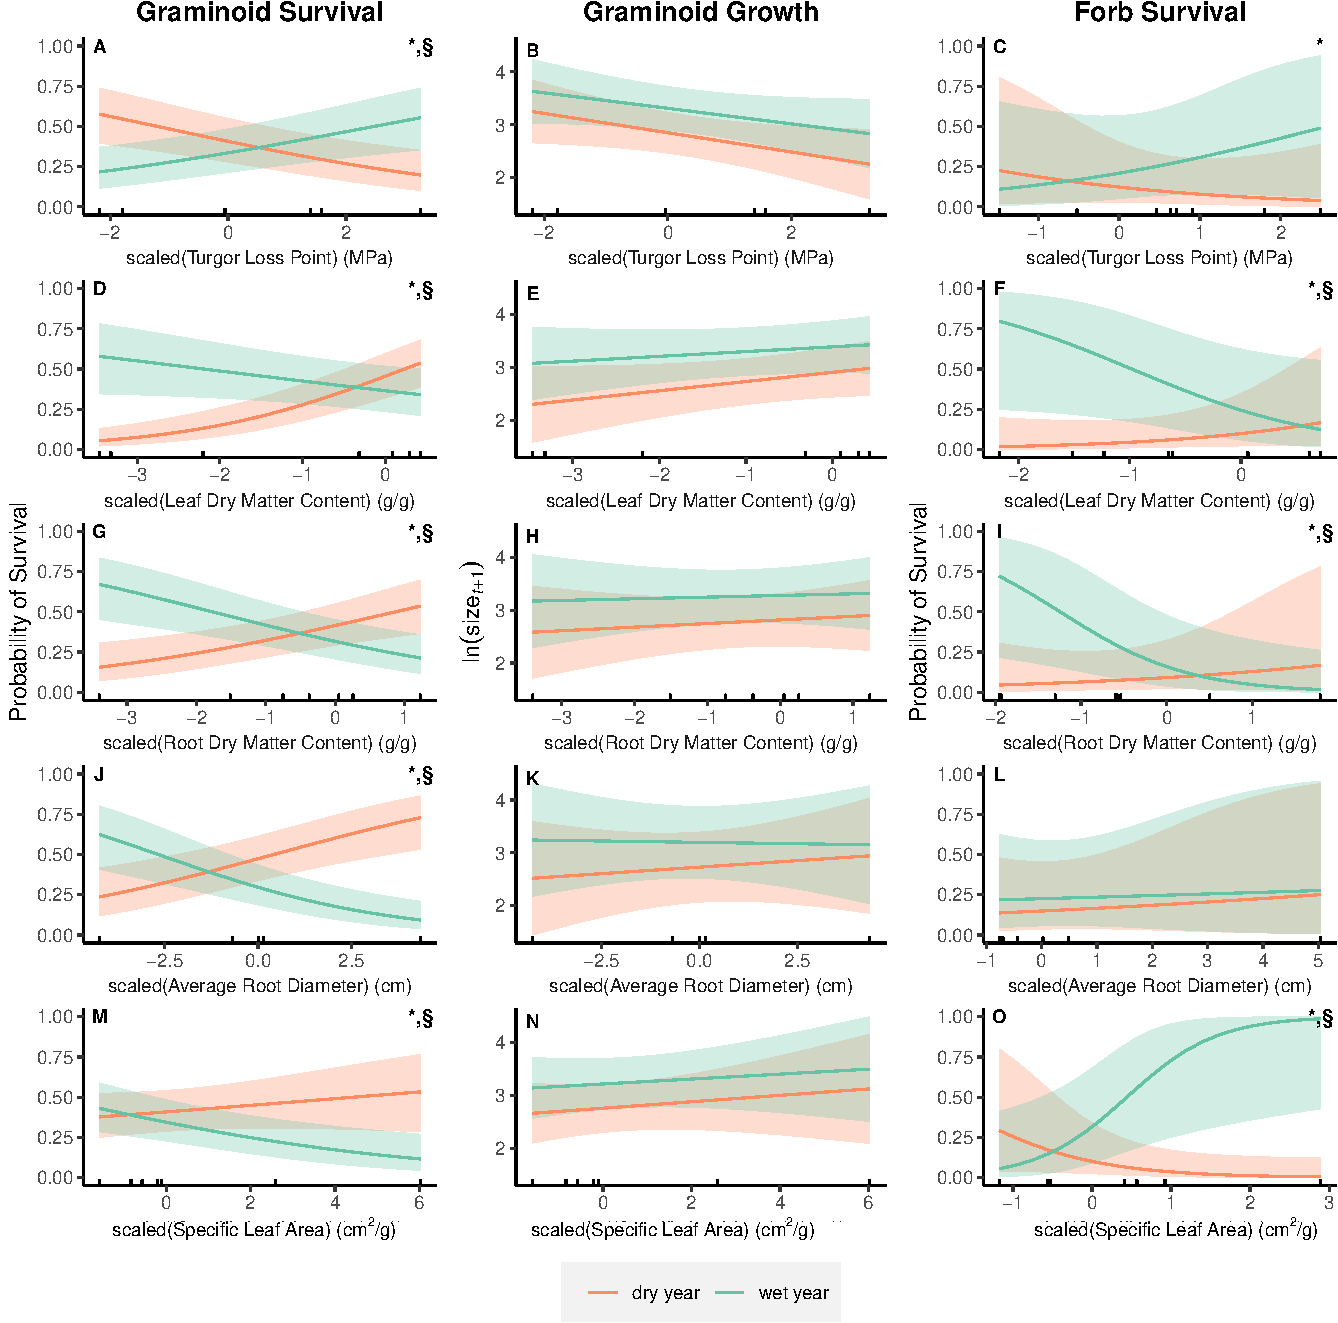
\includegraphics{figures/mainObservationsFig-1.pdf}

Make climate variability figure for use in the conceptual diagram
(fig.~1)

\begin{Shaded}
\begin{Highlighting}[]
\KeywordTok{source}\NormalTok{(}\StringTok{"/Users/Alice/Dropbox/Grad School/Research/Trait Project/Data/Climate Data/CrossSiteClimateComparison.R"}\NormalTok{)}


\CommentTok{\#figure of annual precip variability at CO site}
\NormalTok{CO\_precip \textless{}{-}}\StringTok{ }\KeywordTok{ggplot}\NormalTok{(}\DataTypeTok{data =}\NormalTok{ CO[}\OperatorTok{!}\KeywordTok{is.na}\NormalTok{(CO}\OperatorTok{$}\NormalTok{Ann.Sum.Precip),])}\OperatorTok{+}
\StringTok{  }\KeywordTok{geom\_line}\NormalTok{(}\KeywordTok{aes}\NormalTok{(}\DataTypeTok{x =}\NormalTok{ Year, }\DataTypeTok{y =}\NormalTok{ Ann.Sum.Precip), }\DataTypeTok{col =} \StringTok{"gray25"}\NormalTok{) }\OperatorTok{+}
\StringTok{  }\KeywordTok{ylab}\NormalTok{(}\KeywordTok{expression}\NormalTok{(}\StringTok{"MAP (mm)"} \OperatorTok{\%{-}\textgreater{}\%}\StringTok{ ""}\NormalTok{)) }\OperatorTok{+}\StringTok{ }
\StringTok{  }\KeywordTok{scale\_x\_continuous}\NormalTok{(}\DataTypeTok{labels =} \OtherTok{NULL}\NormalTok{, }\DataTypeTok{breaks =} \OtherTok{NULL}\NormalTok{) }\OperatorTok{+}\StringTok{ }
\StringTok{  }\KeywordTok{scale\_y\_continuous}\NormalTok{(}\DataTypeTok{labels =} \OtherTok{NULL}\NormalTok{, }\DataTypeTok{breaks =} \OtherTok{NULL}\NormalTok{) }\OperatorTok{+}
\StringTok{  }\KeywordTok{theme\_classic}\NormalTok{() }

\KeywordTok{setwd}\NormalTok{(}\StringTok{"/Users/Alice/Dropbox/Grad School/Research/Trait Project/CO\_sgs Analysis"}\NormalTok{)}
\KeywordTok{pdf}\NormalTok{(}\StringTok{"./Manuscript/Figures/CO\_MAP.pdf"}\NormalTok{, }\DataTypeTok{width =} \DecValTok{3}\NormalTok{, }\DataTypeTok{height =} \DecValTok{3}\NormalTok{)}
\NormalTok{CO\_precip}
\KeywordTok{dev.off}\NormalTok{()}
\end{Highlighting}
\end{Shaded}

\begin{verbatim}
## pdf 
##   2
\end{verbatim}

Make a plot of random effects of individual plant size on survival for
LDMC model (best model for graminoid survival)

\begin{Shaded}
\begin{Highlighting}[]
\CommentTok{\#get random effect data}
\CommentTok{\#refit model w/ factors instead of logical values}
\NormalTok{m2\_fac \textless{}{-}}\StringTok{ }\KeywordTok{glmer}\NormalTok{(}\KeywordTok{as.factor}\NormalTok{(survives\_tplus1) }\OperatorTok{\textasciitilde{}}\StringTok{ }\NormalTok{SPEI\_s }\OperatorTok{*}\StringTok{ }\NormalTok{LDMC\_s }\OperatorTok{+}\StringTok{  }\NormalTok{area\_s }\OperatorTok{+}\StringTok{ }\NormalTok{neighbors\_}\DecValTok{10}\NormalTok{\_s }\OperatorTok{+}\StringTok{ }\KeywordTok{as.factor}\NormalTok{(nearEdge\_t) }\OperatorTok{+}\StringTok{ }\NormalTok{(area\_s}\OperatorTok{|}\NormalTok{species) }\OperatorTok{+}\StringTok{ }\NormalTok{(}\DecValTok{1}\OperatorTok{|}\NormalTok{quad) }\OperatorTok{+}\StringTok{ }\NormalTok{(}\DecValTok{1}\OperatorTok{|}\NormalTok{year\_t), }\DataTypeTok{data=}\NormalTok{CO\_poly\_LDMC, }\DataTypeTok{family =} \KeywordTok{binomial}\NormalTok{(}\DataTypeTok{link =}\NormalTok{ logit), }\DataTypeTok{control=}\KeywordTok{glmerControl}\NormalTok{(}\DataTypeTok{optimizer=}\StringTok{"bobyqa"}\NormalTok{))}

\NormalTok{sppAreaPreds\_s \textless{}{-}}\StringTok{ }\KeywordTok{ggpredict}\NormalTok{(m2\_fac, }\DataTypeTok{terms =} \KeywordTok{c}\NormalTok{(}\StringTok{"area\_s[all]"}\NormalTok{, }\StringTok{"species"}\NormalTok{), }\DataTypeTok{type =} \StringTok{"random"}\NormalTok{)}
\NormalTok{sppAreaPreds\_s \textless{}{-}}\StringTok{ }\KeywordTok{data.frame}\NormalTok{(}\StringTok{"x"}\NormalTok{ =}\StringTok{ }\NormalTok{sppAreaPreds\_s}\OperatorTok{$}\NormalTok{x, }\StringTok{"preds"}\NormalTok{ =}\StringTok{ }\NormalTok{sppAreaPreds\_s}\OperatorTok{$}\NormalTok{predicted,}\StringTok{"spp"}\NormalTok{ =}\StringTok{ }\NormalTok{sppAreaPreds\_s}\OperatorTok{$}\NormalTok{group )}

\NormalTok{globPreds\_a\_s \textless{}{-}}\StringTok{ }\KeywordTok{ggpredict}\NormalTok{(m2\_fac, }\DataTypeTok{terms =} \KeywordTok{c}\NormalTok{(}\StringTok{"area\_s[all]"}\NormalTok{), }\DataTypeTok{type =} \StringTok{"random"}\NormalTok{)}
\NormalTok{globPreds\_a\_s \textless{}{-}}\StringTok{ }\KeywordTok{data.frame}\NormalTok{(}\StringTok{"x"}\NormalTok{ =}\StringTok{ }\NormalTok{globPreds\_a\_s}\OperatorTok{$}\NormalTok{x, }\StringTok{"preds"}\NormalTok{ =}\StringTok{ }\NormalTok{globPreds\_a\_s}\OperatorTok{$}\NormalTok{predicted, }\StringTok{"spp"}\NormalTok{ =}\StringTok{ }\KeywordTok{as.factor}\NormalTok{(}\StringTok{"Global"}\NormalTok{), }\StringTok{"CI\_low"}\NormalTok{ =}\StringTok{ }\NormalTok{globPreds\_a\_s}\OperatorTok{$}\NormalTok{conf.low, }\StringTok{"CI\_high"}\NormalTok{ =}\StringTok{ }\NormalTok{globPreds\_a\_s}\OperatorTok{$}\NormalTok{conf.high)}

\NormalTok{AreaEffectSurv \textless{}{-}}\StringTok{ }\KeywordTok{ggplot}\NormalTok{() }\OperatorTok{+}
\StringTok{  }\KeywordTok{geom\_line}\NormalTok{(}\DataTypeTok{data =}\NormalTok{ sppAreaPreds\_s, }\KeywordTok{aes}\NormalTok{(}\DataTypeTok{x =}\NormalTok{ x, }\DataTypeTok{y =}\NormalTok{ preds, }\DataTypeTok{col =}\NormalTok{ spp), }\DataTypeTok{alpha =} \FloatTok{.8}\NormalTok{)}\OperatorTok{+}
\StringTok{  }\KeywordTok{geom\_line}\NormalTok{(}\DataTypeTok{data =}\NormalTok{ globPreds\_a\_s, }\KeywordTok{aes}\NormalTok{(}\DataTypeTok{x =}\NormalTok{ x, }\DataTypeTok{y =}\NormalTok{ preds), }\DataTypeTok{lwd =} \FloatTok{1.25}\NormalTok{) }\OperatorTok{+}
\StringTok{  }\CommentTok{\#geom\_line(aes(x = globPreds\_a\_s$x, y = globPreds\_a\_s$CI\_low)) +}
\StringTok{  }\KeywordTok{geom\_polygon}\NormalTok{(}\KeywordTok{aes}\NormalTok{(}\DataTypeTok{x =} \KeywordTok{c}\NormalTok{(globPreds\_a\_s}\OperatorTok{$}\NormalTok{x,}\KeywordTok{rev}\NormalTok{(globPreds\_a\_s}\OperatorTok{$}\NormalTok{x)), }\DataTypeTok{y =} \KeywordTok{c}\NormalTok{( globPreds\_a\_s}\OperatorTok{$}\NormalTok{CI\_low, }\KeywordTok{rev}\NormalTok{(globPreds\_a\_s}\OperatorTok{$}\NormalTok{CI\_high))), }\DataTypeTok{col =} \OtherTok{NA}\NormalTok{, }\DataTypeTok{fill =} \StringTok{"grey"}\NormalTok{, }\DataTypeTok{alpha =} \FloatTok{.2}\NormalTok{) }\OperatorTok{+}
\StringTok{  }\KeywordTok{theme\_classic}\NormalTok{() }\OperatorTok{+}
\StringTok{  }\KeywordTok{xlab}\NormalTok{(}\KeywordTok{c}\NormalTok{(}\KeywordTok{expression}\NormalTok{(size[year\_t] ))) }\OperatorTok{+}
\StringTok{  }\KeywordTok{ylab}\NormalTok{(}\StringTok{"P(Graminoid Survival)"}\NormalTok{) }\OperatorTok{+}
\StringTok{  }\KeywordTok{scale\_color\_manual}\NormalTok{(}\DataTypeTok{values =} \KeywordTok{c}\NormalTok{(}\StringTok{"grey60"}\NormalTok{, }\StringTok{"grey60"}\NormalTok{, }\StringTok{"grey60"}\NormalTok{, }\StringTok{"grey60"}\NormalTok{, }\StringTok{"grey60"}\NormalTok{, }\StringTok{"grey60"}\NormalTok{, }\StringTok{"grey60"}\NormalTok{, }\StringTok{"grey60"}\NormalTok{)) }\OperatorTok{+}
\StringTok{  }\KeywordTok{theme}\NormalTok{(}\DataTypeTok{axis.ticks.x.bottom =} \KeywordTok{element\_blank}\NormalTok{(),}
        \DataTypeTok{axis.text.x.bottom =} \KeywordTok{element\_blank}\NormalTok{(),}
        \DataTypeTok{legend.position =} \StringTok{"none"}\NormalTok{)}
\end{Highlighting}
\end{Shaded}

Make plot of fixed effect of neighborhood density for effect of
LDMC*SPEI on graminoid survival

\begin{Shaded}
\begin{Highlighting}[]
\NormalTok{sppNeighPreds\_s \textless{}{-}}\StringTok{ }\KeywordTok{ggpredict}\NormalTok{(m2\_fac, }\DataTypeTok{terms =} \KeywordTok{c}\NormalTok{(}\StringTok{"neighbors\_10\_s[all]"}\NormalTok{, }\StringTok{"species"}\NormalTok{), }\DataTypeTok{type =} \StringTok{"random"}\NormalTok{)}
\NormalTok{sppNeighPreds\_s \textless{}{-}}\StringTok{ }\KeywordTok{data.frame}\NormalTok{(}\StringTok{"x"}\NormalTok{ =}\StringTok{ }\NormalTok{sppNeighPreds\_s}\OperatorTok{$}\NormalTok{x, }\StringTok{"preds"}\NormalTok{ =}\StringTok{ }\NormalTok{sppNeighPreds\_s}\OperatorTok{$}\NormalTok{predicted,}\StringTok{"spp"}\NormalTok{ =}\StringTok{ }\NormalTok{sppNeighPreds\_s}\OperatorTok{$}\NormalTok{group )}

\NormalTok{globPreds\_n\_s \textless{}{-}}\StringTok{ }\KeywordTok{ggpredict}\NormalTok{(m2\_fac, }\DataTypeTok{terms =} \KeywordTok{c}\NormalTok{(}\StringTok{"neighbors\_10\_s[all]"}\NormalTok{), }\DataTypeTok{type =} \StringTok{"fixed"}\NormalTok{)}
\NormalTok{globPreds\_n\_s \textless{}{-}}\StringTok{ }\KeywordTok{data.frame}\NormalTok{(}\StringTok{"x"}\NormalTok{ =}\StringTok{ }\NormalTok{globPreds\_n\_s}\OperatorTok{$}\NormalTok{x, }\StringTok{"preds"}\NormalTok{ =}\StringTok{ }\NormalTok{globPreds\_n\_s}\OperatorTok{$}\NormalTok{predicted, }\StringTok{"spp"}\NormalTok{ =}\StringTok{ }\KeywordTok{as.factor}\NormalTok{(}\StringTok{"Global"}\NormalTok{), }\StringTok{"CI\_low"}\NormalTok{ =}\StringTok{ }\NormalTok{globPreds\_n\_s}\OperatorTok{$}\NormalTok{conf.low, }\StringTok{"CI\_high"}\NormalTok{ =}\StringTok{ }\NormalTok{globPreds\_n\_s}\OperatorTok{$}\NormalTok{conf.high)}

\NormalTok{NeighEffectSurv \textless{}{-}}\StringTok{ }\KeywordTok{ggplot}\NormalTok{() }\OperatorTok{+}
\StringTok{  }\KeywordTok{geom\_line}\NormalTok{(}\DataTypeTok{data =}\NormalTok{ sppNeighPreds\_s, }\KeywordTok{aes}\NormalTok{(}\DataTypeTok{x =}\NormalTok{ x, }\DataTypeTok{y =}\NormalTok{ preds, }\DataTypeTok{col =}\NormalTok{ spp), }\DataTypeTok{alpha =} \FloatTok{.8}\NormalTok{)}\OperatorTok{+}
\StringTok{  }\KeywordTok{geom\_line}\NormalTok{(}\DataTypeTok{data =}\NormalTok{ globPreds\_n\_s, }\KeywordTok{aes}\NormalTok{(}\DataTypeTok{x =}\NormalTok{ x, }\DataTypeTok{y =}\NormalTok{ preds), }\DataTypeTok{lwd =} \FloatTok{1.25}\NormalTok{) }\OperatorTok{+}
\StringTok{  }\KeywordTok{geom\_polygon}\NormalTok{(}\KeywordTok{aes}\NormalTok{(}\DataTypeTok{x =} \KeywordTok{c}\NormalTok{(globPreds\_n\_s}\OperatorTok{$}\NormalTok{x,}\KeywordTok{rev}\NormalTok{(globPreds\_n\_s}\OperatorTok{$}\NormalTok{x)), }\DataTypeTok{y =} \KeywordTok{c}\NormalTok{( globPreds\_n\_s}\OperatorTok{$}\NormalTok{CI\_low, }\KeywordTok{rev}\NormalTok{(globPreds\_n\_s}\OperatorTok{$}\NormalTok{CI\_high))), }\DataTypeTok{col =} \OtherTok{NA}\NormalTok{, }\DataTypeTok{fill =} \StringTok{"grey"}\NormalTok{, }\DataTypeTok{alpha =} \FloatTok{.2}\NormalTok{) }\OperatorTok{+}
\StringTok{  }\KeywordTok{theme\_classic}\NormalTok{() }\OperatorTok{+}
\StringTok{  }\KeywordTok{ylim}\NormalTok{(}\KeywordTok{c}\NormalTok{(}\DecValTok{0}\NormalTok{,}\DecValTok{1}\NormalTok{))}\OperatorTok{+}
\StringTok{  }\KeywordTok{xlab}\NormalTok{(}\StringTok{"Conspecific Local Neighborhood Competition"}\NormalTok{) }\OperatorTok{+}
\StringTok{  }\KeywordTok{ylab}\NormalTok{(}\StringTok{"P(Graminoid Survival)"}\NormalTok{) }\OperatorTok{+}
\StringTok{  }\KeywordTok{scale\_color\_manual}\NormalTok{(}\DataTypeTok{values =} \KeywordTok{c}\NormalTok{(}\StringTok{"grey60"}\NormalTok{, }\StringTok{"grey60"}\NormalTok{, }\StringTok{"grey60"}\NormalTok{, }\StringTok{"grey60"}\NormalTok{, }\StringTok{"grey60"}\NormalTok{, }\StringTok{"grey60"}\NormalTok{, }\StringTok{"grey60"}\NormalTok{, }\StringTok{"grey60"}\NormalTok{)) }\OperatorTok{+}
\StringTok{  }\KeywordTok{theme}\NormalTok{(}\DataTypeTok{axis.ticks.x.bottom =} \KeywordTok{element\_blank}\NormalTok{(),}
        \DataTypeTok{axis.text.x.bottom =} \KeywordTok{element\_blank}\NormalTok{(),}
        \DataTypeTok{legend.position =} \StringTok{"none"}\NormalTok{)}
\end{Highlighting}
\end{Shaded}

Make plot of fixed effect of neighborhood by species on growth for TLP
model

\begin{Shaded}
\begin{Highlighting}[]
\NormalTok{mGrowTLP\_fac\textless{}{-}}\StringTok{ }\NormalTok{lme4}\OperatorTok{::}\KeywordTok{lmer}\NormalTok{(logDiffArea }\OperatorTok{\textasciitilde{}}\StringTok{  }\NormalTok{neighbors\_}\DecValTok{10}\NormalTok{\_s }\OperatorTok{+}\StringTok{ }\NormalTok{TLP\_s }\OperatorTok{+}\StringTok{ }\NormalTok{SPEI\_s }\OperatorTok{*}\StringTok{ }\NormalTok{TLP\_s }\OperatorTok{+}\StringTok{ }\KeywordTok{as.factor}\NormalTok{(nearEdge\_t) }\OperatorTok{+}\StringTok{ }\NormalTok{(}\DecValTok{1}\OperatorTok{|}\NormalTok{species) }\OperatorTok{+}\StringTok{ }\NormalTok{(}\DecValTok{1}\OperatorTok{|}\NormalTok{quad) }\OperatorTok{+}\StringTok{ }\NormalTok{(}\DecValTok{1}\OperatorTok{|}\NormalTok{year\_t), }\DataTypeTok{data =}\NormalTok{ CO\_grow\_TLP , }\DataTypeTok{control=}\KeywordTok{lmerControl}\NormalTok{(}\DataTypeTok{optimizer=}\StringTok{"bobyqa"}\NormalTok{))}

\NormalTok{sppNeighPreds\_g \textless{}{-}}\StringTok{ }\KeywordTok{ggpredict}\NormalTok{(mGrowTLP\_fac, }\DataTypeTok{terms =} \KeywordTok{c}\NormalTok{(}\StringTok{"neighbors\_10\_s[all]"}\NormalTok{, }\StringTok{"species"}\NormalTok{), }\DataTypeTok{type =} \StringTok{"random"}\NormalTok{)}
\NormalTok{sppNeighPreds\_g \textless{}{-}}\StringTok{ }\KeywordTok{data.frame}\NormalTok{(}\StringTok{"x"}\NormalTok{ =}\StringTok{ }\NormalTok{sppNeighPreds\_g}\OperatorTok{$}\NormalTok{x, }\StringTok{"preds"}\NormalTok{ =}\StringTok{ }\NormalTok{sppNeighPreds\_g}\OperatorTok{$}\NormalTok{predicted,}\StringTok{"spp"}\NormalTok{ =}\StringTok{ }\NormalTok{sppNeighPreds\_g}\OperatorTok{$}\NormalTok{group )}

\NormalTok{globPreds\_n\_g \textless{}{-}}\StringTok{ }\KeywordTok{ggpredict}\NormalTok{(mGrowTLP\_fac, }\DataTypeTok{terms =} \KeywordTok{c}\NormalTok{(}\StringTok{"neighbors\_10\_s[all]"}\NormalTok{), }\DataTypeTok{type =} \StringTok{"fixed"}\NormalTok{)}
\NormalTok{globPreds\_n\_g \textless{}{-}}\StringTok{ }\KeywordTok{data.frame}\NormalTok{(}\StringTok{"x"}\NormalTok{ =}\StringTok{ }\NormalTok{globPreds\_n\_g}\OperatorTok{$}\NormalTok{x, }\StringTok{"preds"}\NormalTok{ =}\StringTok{ }\NormalTok{globPreds\_n\_g}\OperatorTok{$}\NormalTok{predicted, }\StringTok{"spp"}\NormalTok{ =}\StringTok{ }\KeywordTok{as.factor}\NormalTok{(}\StringTok{"Global"}\NormalTok{), }\StringTok{"CI\_low"}\NormalTok{ =}\StringTok{ }\NormalTok{globPreds\_n\_g}\OperatorTok{$}\NormalTok{conf.low, }\StringTok{"CI\_high"}\NormalTok{ =}\StringTok{ }\NormalTok{globPreds\_n\_g}\OperatorTok{$}\NormalTok{conf.high)}

\NormalTok{NeighEffectGrowth \textless{}{-}}\StringTok{ }\KeywordTok{ggplot}\NormalTok{() }\OperatorTok{+}
\StringTok{  }\KeywordTok{geom\_line}\NormalTok{(}\DataTypeTok{data =}\NormalTok{ sppNeighPreds\_g, }\KeywordTok{aes}\NormalTok{(}\DataTypeTok{x =}\NormalTok{ x, }\DataTypeTok{y =}\NormalTok{ preds, }\DataTypeTok{col =}\NormalTok{ spp), }\DataTypeTok{alpha =} \FloatTok{.8}\NormalTok{)}\OperatorTok{+}
\StringTok{  }\KeywordTok{geom\_line}\NormalTok{(}\DataTypeTok{data =}\NormalTok{ globPreds\_n\_g, }\KeywordTok{aes}\NormalTok{(}\DataTypeTok{x =}\NormalTok{ x, }\DataTypeTok{y =}\NormalTok{ preds), }\DataTypeTok{lwd =} \FloatTok{1.25}\NormalTok{) }\OperatorTok{+}
\StringTok{  }\KeywordTok{geom\_polygon}\NormalTok{(}\KeywordTok{aes}\NormalTok{(}\DataTypeTok{x =} \KeywordTok{c}\NormalTok{(globPreds\_n\_g}\OperatorTok{$}\NormalTok{x,}\KeywordTok{rev}\NormalTok{(globPreds\_n\_g}\OperatorTok{$}\NormalTok{x)), }\DataTypeTok{y =} \KeywordTok{c}\NormalTok{( globPreds\_n\_g}\OperatorTok{$}\NormalTok{CI\_low, }\KeywordTok{rev}\NormalTok{(globPreds\_n\_g}\OperatorTok{$}\NormalTok{CI\_high))), }\DataTypeTok{col =} \OtherTok{NA}\NormalTok{, }\DataTypeTok{fill =} \StringTok{"grey"}\NormalTok{, }\DataTypeTok{alpha =} \FloatTok{.2}\NormalTok{) }\OperatorTok{+}
\StringTok{  }\KeywordTok{theme\_classic}\NormalTok{() }\OperatorTok{+}
\StringTok{  }\KeywordTok{xlab}\NormalTok{(}\KeywordTok{c}\NormalTok{(}\KeywordTok{expression}\NormalTok{(}\StringTok{"Conspecific Local Neighborhood Competition"}\NormalTok{))) }\OperatorTok{+}
\StringTok{  }\KeywordTok{ylab}\NormalTok{(}\KeywordTok{expression}\NormalTok{(}\StringTok{"log"} \OperatorTok{\textasciitilde{}}\StringTok{ }\KeywordTok{bgroup}\NormalTok{(}\StringTok{"("}\NormalTok{,}\KeywordTok{frac}\NormalTok{(size[year\_t}\OperatorTok{+}\DecValTok{1}\NormalTok{],size[year\_t]),}\StringTok{")"}\NormalTok{))) }\OperatorTok{+}
\StringTok{  }\KeywordTok{scale\_color\_manual}\NormalTok{(}\DataTypeTok{values =} \KeywordTok{c}\NormalTok{(}\StringTok{"grey60"}\NormalTok{, }\StringTok{"grey60"}\NormalTok{, }\StringTok{"grey60"}\NormalTok{, }\StringTok{"grey60"}\NormalTok{, }\StringTok{"grey60"}\NormalTok{, }\StringTok{"grey60"}\NormalTok{, }\StringTok{"grey60"}\NormalTok{, }\StringTok{"grey60"}\NormalTok{)) }\OperatorTok{+}
\StringTok{  }\KeywordTok{theme}\NormalTok{(}\DataTypeTok{axis.ticks =} \KeywordTok{element\_blank}\NormalTok{(),}
        \DataTypeTok{axis.text =} \KeywordTok{element\_blank}\NormalTok{(),}
        \DataTypeTok{legend.position =} \StringTok{"none"}\NormalTok{) }
\end{Highlighting}
\end{Shaded}

Make figure 3 (combination of figures for effect of size and local
neighborhood on LDMC*SPEI effect of graminoid survival)

\begin{Shaded}
\begin{Highlighting}[]
\NormalTok{(effectsSurv \textless{}{-}}\StringTok{ }\KeywordTok{ggarrange}\NormalTok{(AreaEffectSurv, NeighEffectSurv,}
          \DataTypeTok{labels =} \KeywordTok{c}\NormalTok{(}\StringTok{"A"}\NormalTok{, }\StringTok{"B"}\NormalTok{),}
          \DataTypeTok{ncol =} \DecValTok{2}\NormalTok{, }\DataTypeTok{nrow =} \DecValTok{1}\NormalTok{))}
\end{Highlighting}
\end{Shaded}

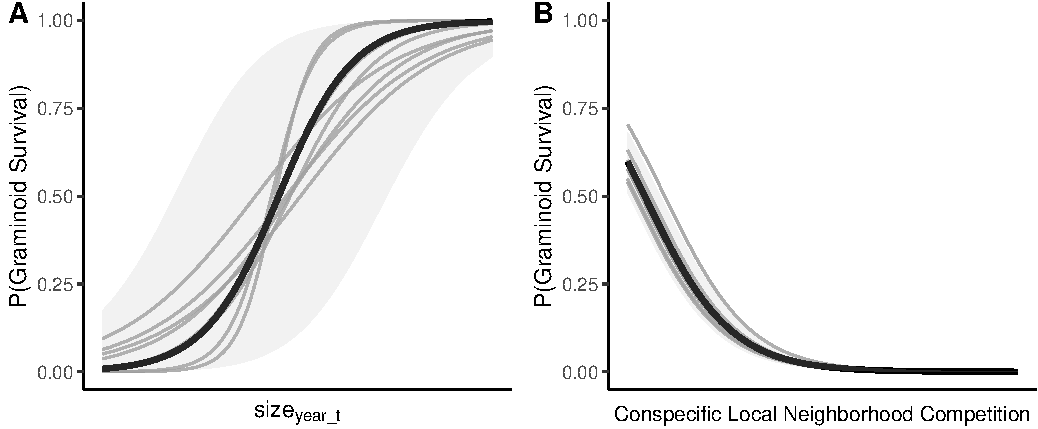
\includegraphics{figures/survEffectPlots-1.pdf}

Make figure 7 in supplement (figure for effect of local neighborhood on
TLP*SPEI effect of graminoid growth)

\begin{Shaded}
\begin{Highlighting}[]
\NormalTok{(effectsGrowth \textless{}{-}}\StringTok{ }\NormalTok{NeighEffectGrowth)}
\end{Highlighting}
\end{Shaded}

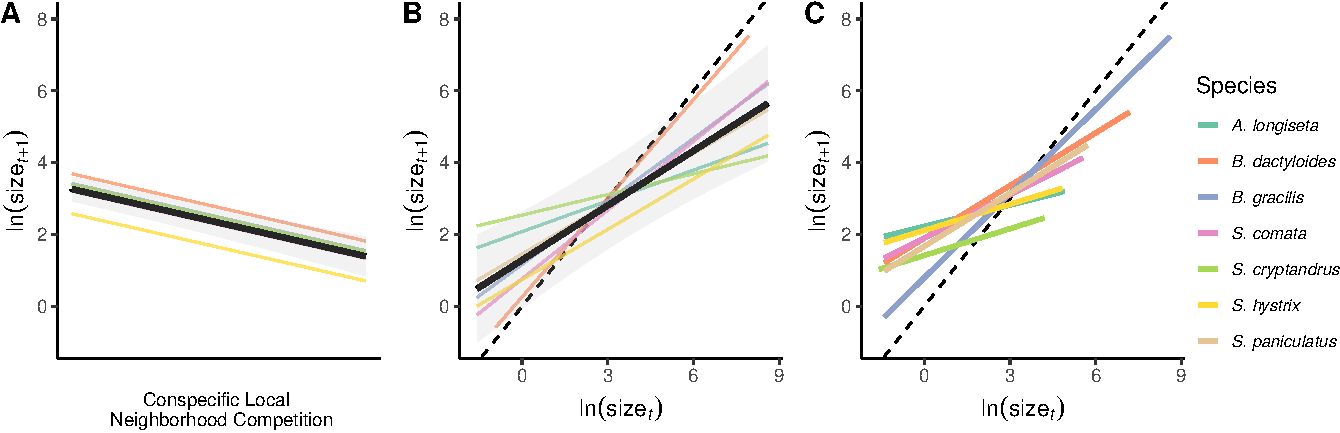
\includegraphics{figures/growthEffectPlots-1.pdf}

plot of all graminoid survival model results (for traits not in fig.~2)

\begin{Shaded}
\begin{Highlighting}[]
\CommentTok{\#\#polygons}
\CommentTok{\#TLP}
\CommentTok{\#get 2.5 and 97.5 percentiles of the distribution}
\NormalTok{meanSPEI\_G \textless{}{-}}\StringTok{ }\KeywordTok{mean}\NormalTok{(CO\_grams}\OperatorTok{$}\NormalTok{SPEI\_s)}
\NormalTok{sdSPEI\_G \textless{}{-}}\StringTok{ }\KeywordTok{sd}\NormalTok{(CO\_grams}\OperatorTok{$}\NormalTok{SPEI\_s)}
\CommentTok{\#get 97.5 quantile of the distribution}
\NormalTok{SPEI\_}\DecValTok{97}\NormalTok{\_}\DecValTok{5}\NormalTok{\_G \textless{}{-}}\StringTok{ }\KeywordTok{qnorm}\NormalTok{(.}\DecValTok{975}\NormalTok{, meanSPEI\_G, sdSPEI\_G) }\CommentTok{\#2.10}
\NormalTok{SPEI\_}\DecValTok{2}\NormalTok{\_}\DecValTok{5}\NormalTok{\_G \textless{}{-}}\StringTok{ }\KeywordTok{qnorm}\NormalTok{(.}\DecValTok{025}\NormalTok{, meanSPEI\_G, sdSPEI\_G) }\CommentTok{\#{-}1.48}

\NormalTok{spei\_vals \textless{}{-}}\StringTok{ }\KeywordTok{c}\NormalTok{(SPEI\_}\DecValTok{2}\NormalTok{\_}\DecValTok{5}\NormalTok{\_G, SPEI\_}\DecValTok{97}\NormalTok{\_}\DecValTok{5}\NormalTok{\_G)}
\NormalTok{SLA\_vals \textless{}{-}}\StringTok{ }\KeywordTok{seq}\NormalTok{(}\KeywordTok{min}\NormalTok{(CO\_grams}\OperatorTok{$}\NormalTok{SLA\_s), }\KeywordTok{max}\NormalTok{(CO\_grams}\OperatorTok{$}\NormalTok{SLA\_s), }\DataTypeTok{length.out =} \DecValTok{20}\NormalTok{)}

\NormalTok{SLA\_G\_dat \textless{}{-}}\StringTok{ }\KeywordTok{ggpredict}\NormalTok{(m5, }\DataTypeTok{terms =} \KeywordTok{c}\NormalTok{(}\StringTok{"SLA\_s[SLA\_vals]"}\NormalTok{, }\StringTok{"SPEI\_s[spei\_vals]"}\NormalTok{), }\DataTypeTok{type =} \StringTok{"fixed"}\NormalTok{, }\DataTypeTok{back.transform =} \OtherTok{TRUE}\NormalTok{)}

\CommentTok{\#for RTD\_s}
\NormalTok{RTD\_vals \textless{}{-}}\StringTok{ }\KeywordTok{seq}\NormalTok{(}\KeywordTok{min}\NormalTok{(CO\_grams}\OperatorTok{$}\NormalTok{RTD\_s, }\DataTypeTok{na.rm =} \OtherTok{TRUE}\NormalTok{), }\KeywordTok{max}\NormalTok{(CO\_grams}\OperatorTok{$}\NormalTok{RTD\_s, }\DataTypeTok{na.rm =} \OtherTok{TRUE}\NormalTok{), }\DataTypeTok{length.out =} \DecValTok{20}\NormalTok{)}
\NormalTok{RTD\_G\_dat \textless{}{-}}\StringTok{ }\KeywordTok{ggpredict}\NormalTok{(m10, }\DataTypeTok{terms =} \KeywordTok{c}\NormalTok{(}\StringTok{"RTD\_s[RTD\_vals]"}\NormalTok{, }\StringTok{"SPEI\_s[spei\_vals]"}\NormalTok{), }\DataTypeTok{type =} \StringTok{"fixed"}\NormalTok{, }\DataTypeTok{back.transform =} \OtherTok{TRUE}\NormalTok{)}

\CommentTok{\#for SRL\_s}
\NormalTok{SRL\_vals \textless{}{-}}\StringTok{ }\KeywordTok{seq}\NormalTok{(}\KeywordTok{min}\NormalTok{(CO\_grams}\OperatorTok{$}\NormalTok{SRL\_s, }\DataTypeTok{na.rm =} \OtherTok{TRUE}\NormalTok{), }\KeywordTok{max}\NormalTok{(CO\_grams}\OperatorTok{$}\NormalTok{SRL\_s, }\DataTypeTok{na.rm =} \OtherTok{TRUE}\NormalTok{), }\DataTypeTok{length.out =} \DecValTok{20}\NormalTok{)}
\NormalTok{SRL\_G\_dat \textless{}{-}}\StringTok{ }\KeywordTok{ggpredict}\NormalTok{(m13, }\DataTypeTok{terms =} \KeywordTok{c}\NormalTok{(}\StringTok{"SRL\_s[SRL\_vals]"}\NormalTok{, }\StringTok{"SPEI\_s[spei\_vals]"}\NormalTok{), }\DataTypeTok{type =} \StringTok{"fixed"}\NormalTok{, }\DataTypeTok{back.transform =} \OtherTok{TRUE}\NormalTok{)}

\CommentTok{\#for RDiam\_s}
\NormalTok{RDiam\_vals \textless{}{-}}\StringTok{ }\KeywordTok{seq}\NormalTok{(}\KeywordTok{min}\NormalTok{(CO\_grams}\OperatorTok{$}\NormalTok{RDiam\_s, }\DataTypeTok{na.rm =} \OtherTok{TRUE}\NormalTok{), }\KeywordTok{max}\NormalTok{(CO\_grams}\OperatorTok{$}\NormalTok{RDiam\_s, }\DataTypeTok{na.rm =} \OtherTok{TRUE}\NormalTok{), }\DataTypeTok{length.out =} \DecValTok{20}\NormalTok{)}
\NormalTok{RDiam\_G\_dat \textless{}{-}}\StringTok{ }\KeywordTok{ggpredict}\NormalTok{(m14, }\DataTypeTok{terms =} \KeywordTok{c}\NormalTok{(}\StringTok{"RDiam\_s[RDiam\_vals]"}\NormalTok{, }\StringTok{"SPEI\_s[spei\_vals]"}\NormalTok{), }\DataTypeTok{type =} \StringTok{"fixed"}\NormalTok{, }\DataTypeTok{back.transform =} \OtherTok{TRUE}\NormalTok{)}

\CommentTok{\#make a data.frame to contain all of the values for each trait}
\NormalTok{GramDat \textless{}{-}}\StringTok{ }\KeywordTok{data.frame}\NormalTok{(}\DataTypeTok{trait =} \KeywordTok{c}\NormalTok{(}\StringTok{"scaled(Specific Leaf Area)"}\NormalTok{), }\DataTypeTok{x =}\NormalTok{ SLA\_G\_dat}\OperatorTok{$}\NormalTok{x, }\DataTypeTok{GramSurv =}\NormalTok{ SLA\_G\_dat}\OperatorTok{$}\NormalTok{predicted, }\DataTypeTok{CI\_low =}\NormalTok{ SLA\_G\_dat}\OperatorTok{$}\NormalTok{conf.low, }\DataTypeTok{CI\_high =}\NormalTok{ SLA\_G\_dat}\OperatorTok{$}\NormalTok{conf.high, }\DataTypeTok{SPEI =}\NormalTok{ SLA\_G\_dat}\OperatorTok{$}\NormalTok{group, }\DataTypeTok{lab =} \StringTok{"A"}\NormalTok{)}

\NormalTok{GramDat \textless{}{-}}\StringTok{ }\KeywordTok{rbind}\NormalTok{(GramDat, }\KeywordTok{data.frame}\NormalTok{(}\DataTypeTok{trait =} \KeywordTok{c}\NormalTok{(}\StringTok{"scaled(Specific Root Length)"}\NormalTok{), }\DataTypeTok{x =}\NormalTok{ SRL\_G\_dat}\OperatorTok{$}\NormalTok{x, }\DataTypeTok{GramSurv =}\NormalTok{ SRL\_G\_dat}\OperatorTok{$}\NormalTok{predicted, }\DataTypeTok{CI\_low =}\NormalTok{ SRL\_G\_dat}\OperatorTok{$}\NormalTok{conf.low, }\DataTypeTok{CI\_high =}\NormalTok{ SRL\_G\_dat}\OperatorTok{$}\NormalTok{conf.high, }\DataTypeTok{SPEI =}\NormalTok{ SRL\_G\_dat}\OperatorTok{$}\NormalTok{group, }\DataTypeTok{lab =} \StringTok{"B"}\NormalTok{))}
\NormalTok{GramDat \textless{}{-}}\StringTok{ }\KeywordTok{rbind}\NormalTok{(GramDat, }\KeywordTok{data.frame}\NormalTok{(}\DataTypeTok{trait =} \KeywordTok{c}\NormalTok{(}\StringTok{"scaled(Root Tissue Density)"}\NormalTok{), }\DataTypeTok{x =}\NormalTok{ RTD\_G\_dat}\OperatorTok{$}\NormalTok{x, }\DataTypeTok{GramSurv =}\NormalTok{ RTD\_G\_dat}\OperatorTok{$}\NormalTok{predicted, }\DataTypeTok{CI\_low =}\NormalTok{ RTD\_G\_dat}\OperatorTok{$}\NormalTok{conf.low, }\DataTypeTok{CI\_high =}\NormalTok{ RTD\_G\_dat}\OperatorTok{$}\NormalTok{conf.high, }\DataTypeTok{SPEI =}\NormalTok{ RTD\_G\_dat}\OperatorTok{$}\NormalTok{group, }\DataTypeTok{lab =} \StringTok{"C"}\NormalTok{))}
\NormalTok{GramDat \textless{}{-}}\StringTok{ }\KeywordTok{rbind}\NormalTok{(GramDat, }\KeywordTok{data.frame}\NormalTok{(}\DataTypeTok{trait =} \KeywordTok{c}\NormalTok{(}\StringTok{"scaled(Avg. Root Diameter)"}\NormalTok{), }\DataTypeTok{x =}\NormalTok{ RDiam\_G\_dat}\OperatorTok{$}\NormalTok{x, }\DataTypeTok{GramSurv =}\NormalTok{ RDiam\_G\_dat}\OperatorTok{$}\NormalTok{predicted, }\DataTypeTok{CI\_low =}\NormalTok{ RDiam\_G\_dat}\OperatorTok{$}\NormalTok{conf.low, }\DataTypeTok{CI\_high =}\NormalTok{ RDiam\_G\_dat}\OperatorTok{$}\NormalTok{conf.high, }\DataTypeTok{SPEI =}\NormalTok{ RDiam\_G\_dat}\OperatorTok{$}\NormalTok{group, }\DataTypeTok{lab =} \StringTok{"D"}\NormalTok{))}
\CommentTok{\#make data for rug plot}
\NormalTok{RugDat \textless{}{-}}\StringTok{  }\KeywordTok{data.frame}\NormalTok{(}\DataTypeTok{rug =}\NormalTok{ CO\_grams}\OperatorTok{$}\NormalTok{SLA\_s, }\DataTypeTok{trait =} \StringTok{"scaled(Specific Leaf Area)"}\NormalTok{)}
\NormalTok{RugDat \textless{}{-}}\StringTok{ }\KeywordTok{rbind}\NormalTok{(RugDat, }\KeywordTok{data.frame}\NormalTok{(}\DataTypeTok{rug =}\NormalTok{ CO\_grams}\OperatorTok{$}\NormalTok{SRL\_s, }\DataTypeTok{trait =} \StringTok{"scaled(Specific Root Length)"}\NormalTok{))}
\NormalTok{RugDat \textless{}{-}}\StringTok{ }\KeywordTok{rbind}\NormalTok{(RugDat, }\KeywordTok{data.frame}\NormalTok{(}\DataTypeTok{rug =}\NormalTok{ CO\_grams}\OperatorTok{$}\NormalTok{RTD\_s, }\DataTypeTok{trait =} \StringTok{"scaled(Root Tissue Density)"}\NormalTok{))}
\NormalTok{RugDat \textless{}{-}}\StringTok{ }\KeywordTok{rbind}\NormalTok{(RugDat, }\KeywordTok{data.frame}\NormalTok{(}\DataTypeTok{rug =}\NormalTok{ CO\_grams}\OperatorTok{$}\NormalTok{RDiam\_s, }\DataTypeTok{trait =} \StringTok{"scaled(Avg. Root Diameter)"}\NormalTok{))}
\CommentTok{\#text for labels}
\NormalTok{dat\_text \textless{}{-}}\StringTok{ }\KeywordTok{data.frame}\NormalTok{(}
  \DataTypeTok{label =} \KeywordTok{c}\NormalTok{(}\StringTok{"A"}\NormalTok{, }\StringTok{"B"}\NormalTok{, }\StringTok{"C"}\NormalTok{, }\StringTok{"D"}\NormalTok{),}
  \DataTypeTok{trait =} \KeywordTok{c}\NormalTok{(}\StringTok{"scaled(Specific Leaf Area)"}\NormalTok{, }\StringTok{"scaled(Specific Root Length)"}\NormalTok{, }\StringTok{"scaled(Root Tissue Density)"}\NormalTok{, }\StringTok{"scaled(Avg. Root Diameter)"}\NormalTok{),}
  \DataTypeTok{x    =} \KeywordTok{c}\NormalTok{(}\KeywordTok{min}\NormalTok{(SLA\_G\_dat}\OperatorTok{$}\NormalTok{x),}\KeywordTok{min}\NormalTok{(SRL\_G\_dat}\OperatorTok{$}\NormalTok{x),}\KeywordTok{min}\NormalTok{(RTD\_G\_dat}\OperatorTok{$}\NormalTok{x),}\KeywordTok{min}\NormalTok{(RDiam\_G\_dat}\OperatorTok{$}\NormalTok{x)),}
  \DataTypeTok{y     =} \KeywordTok{c}\NormalTok{(}\DecValTok{1}\NormalTok{,}\DecValTok{1}\NormalTok{,}\DecValTok{1}\NormalTok{,}\DecValTok{1}\NormalTok{)}
\NormalTok{)}


\CommentTok{\#make a multipanel figure}
\NormalTok{(GramSurvExtraFig \textless{}{-}}\StringTok{ }\KeywordTok{ggplot}\NormalTok{(}\DataTypeTok{data =}\NormalTok{ GramDat) }\OperatorTok{+}
\StringTok{  }\KeywordTok{geom\_ribbon}\NormalTok{(}\KeywordTok{aes}\NormalTok{(}\DataTypeTok{x =}\NormalTok{ x, }\DataTypeTok{ymin =}\NormalTok{ CI\_low, }\DataTypeTok{ymax =}\NormalTok{ CI\_high, }\DataTypeTok{fill =}\NormalTok{ SPEI), }\DataTypeTok{alpha =} \FloatTok{0.3}\NormalTok{) }\OperatorTok{+}
\StringTok{  }\KeywordTok{geom\_line}\NormalTok{(}\KeywordTok{aes}\NormalTok{(x, GramSurv, }\DataTypeTok{col =}\NormalTok{ SPEI))  }\OperatorTok{+}\StringTok{ }
\StringTok{  }\KeywordTok{geom\_rug}\NormalTok{(}\KeywordTok{aes}\NormalTok{(}\DataTypeTok{x =}\NormalTok{ rug), }\DataTypeTok{data =}\NormalTok{ RugDat) }\OperatorTok{+}
\StringTok{  }\KeywordTok{labs}\NormalTok{(}\DataTypeTok{title =} \OtherTok{NULL}\NormalTok{) }\OperatorTok{+}
\StringTok{  }\KeywordTok{xlab}\NormalTok{(}\OtherTok{NULL}\NormalTok{) }\OperatorTok{+}
\StringTok{  }\KeywordTok{ylab}\NormalTok{(}\StringTok{"P(Graminoid Survival)"}\NormalTok{) }\OperatorTok{+}
\StringTok{  }\KeywordTok{scale\_y\_continuous}\NormalTok{(}\DataTypeTok{limits =} \KeywordTok{c}\NormalTok{(}\DecValTok{0}\NormalTok{,}\DecValTok{1}\NormalTok{)) }\OperatorTok{+}
\StringTok{  }\KeywordTok{scale\_color\_manual}\NormalTok{(}\DataTypeTok{labels =} \KeywordTok{c}\NormalTok{(}\StringTok{"dry year"}\NormalTok{, }\StringTok{"wet year"}\NormalTok{), }\DataTypeTok{values =} \KeywordTok{c}\NormalTok{(}\StringTok{"goldenrod1"}\NormalTok{, }\StringTok{"royalblue2"}\NormalTok{)) }\OperatorTok{+}
\StringTok{  }\KeywordTok{scale\_fill\_manual}\NormalTok{(}\DataTypeTok{values =} \KeywordTok{c}\NormalTok{(}\StringTok{"goldenrod1"}\NormalTok{, }\StringTok{"royalblue2"}\NormalTok{), }\DataTypeTok{guide =} \OtherTok{FALSE}\NormalTok{) }\OperatorTok{+}
\StringTok{  }\KeywordTok{facet\_wrap}\NormalTok{(}\KeywordTok{vars}\NormalTok{(trait), }\DataTypeTok{scales =} \StringTok{"free\_x"}\NormalTok{, }\DataTypeTok{strip.position =}  \StringTok{"bottom"}\NormalTok{) }\OperatorTok{+}
\StringTok{  }\KeywordTok{theme\_classic}\NormalTok{()}\OperatorTok{+}
\StringTok{  }\KeywordTok{theme}\NormalTok{(}\DataTypeTok{legend.position =} \StringTok{"bottom"}\NormalTok{, }\DataTypeTok{legend.title =} \KeywordTok{element\_blank}\NormalTok{(), }\DataTypeTok{legend.background =} \KeywordTok{element\_rect}\NormalTok{(}\DataTypeTok{fill=}\StringTok{"grey95"}\NormalTok{,}\DataTypeTok{size=}\FloatTok{0.5}\NormalTok{, }\DataTypeTok{linetype=}\StringTok{"solid"}\NormalTok{), }\DataTypeTok{strip.background =} \KeywordTok{element\_rect}\NormalTok{(}\DataTypeTok{colour=}\OtherTok{NA}\NormalTok{, }\DataTypeTok{fill=}\OtherTok{NA}\NormalTok{), }\DataTypeTok{strip.placement =} \StringTok{"outside"}\NormalTok{, }\DataTypeTok{strip.text.x =} \KeywordTok{element\_text}\NormalTok{(}\DataTypeTok{margin =} \KeywordTok{margin}\NormalTok{(}\DecValTok{0}\NormalTok{, }\DecValTok{0}\NormalTok{, }\FloatTok{1.5}\NormalTok{, }\DecValTok{0}\NormalTok{))) }\OperatorTok{+}
\StringTok{  }\KeywordTok{geom\_text}\NormalTok{(}\DataTypeTok{data=}\NormalTok{ dat\_text, }\DataTypeTok{mapping =} \KeywordTok{aes}\NormalTok{(}\DataTypeTok{x =}\NormalTok{ x, }\DataTypeTok{y =}\NormalTok{ y, }\DataTypeTok{label =}\NormalTok{ label), }\DataTypeTok{size =} \DecValTok{3}\NormalTok{, }\DataTypeTok{fontface =} \StringTok{"bold"}\NormalTok{))}
\end{Highlighting}
\end{Shaded}

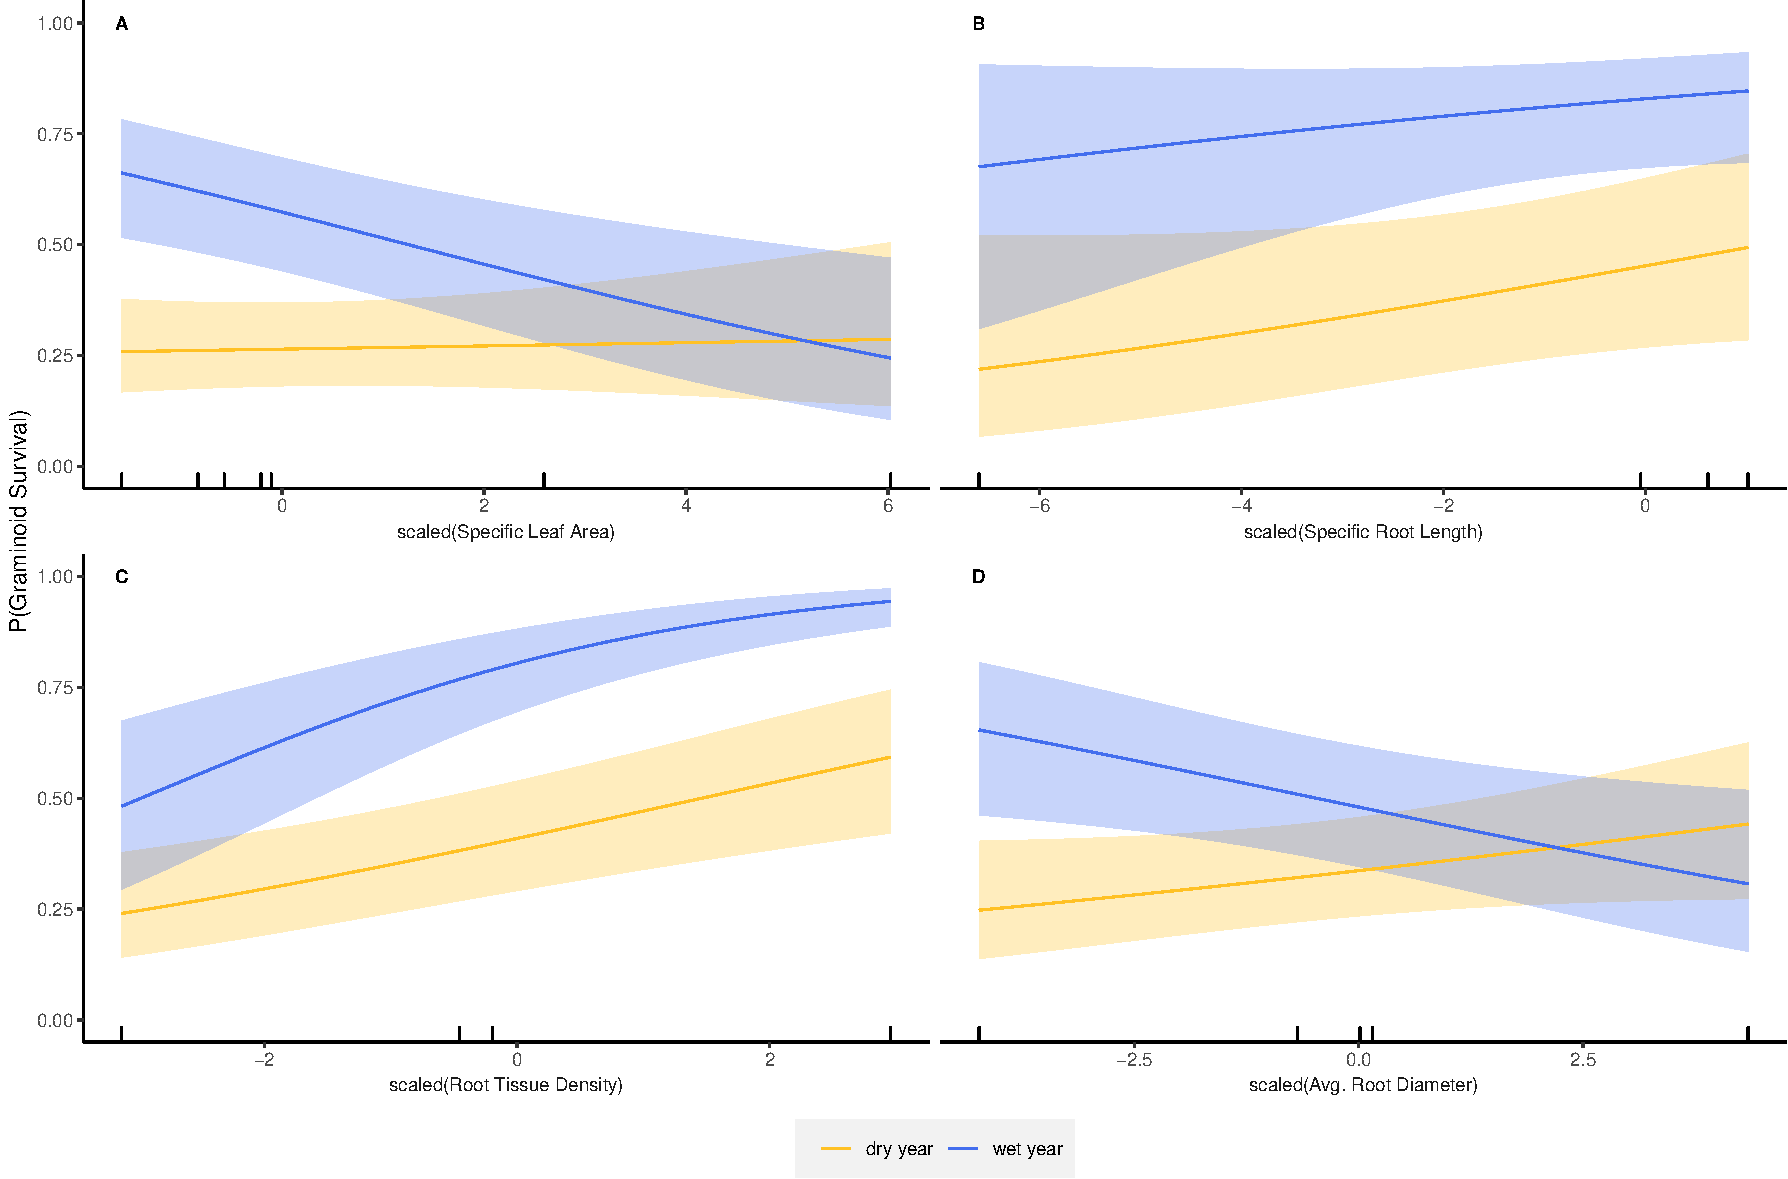
\includegraphics{figures/supGramSurvPlots-1.pdf}

plot of all forb survival model results (for traits not in fig.~2)

\begin{Shaded}
\begin{Highlighting}[]
\CommentTok{\#get 2.5 and 97.5 percentiles of the distribution}
\NormalTok{meanSPEI \textless{}{-}}\StringTok{ }\KeywordTok{mean}\NormalTok{(CO\_point\_all}\OperatorTok{$}\NormalTok{SPEI\_s)}
\NormalTok{sdSPEI \textless{}{-}}\StringTok{ }\KeywordTok{sd}\NormalTok{(CO\_point\_all}\OperatorTok{$}\NormalTok{SPEI\_s)}
\CommentTok{\#get 97.5 quantile of the distribution}
\NormalTok{SPEI\_}\DecValTok{97}\NormalTok{\_}\DecValTok{5}\NormalTok{ \textless{}{-}}\StringTok{ }\KeywordTok{qnorm}\NormalTok{(.}\DecValTok{975}\NormalTok{, meanSPEI, sdSPEI) }
\NormalTok{SPEI\_}\DecValTok{2}\NormalTok{\_}\DecValTok{5}\NormalTok{ \textless{}{-}}\StringTok{ }\KeywordTok{qnorm}\NormalTok{(.}\DecValTok{025}\NormalTok{, meanSPEI, sdSPEI)}

\NormalTok{spei\_vals \textless{}{-}}\StringTok{ }\KeywordTok{c}\NormalTok{(SPEI\_}\DecValTok{2}\NormalTok{\_}\DecValTok{5}\NormalTok{, SPEI\_}\DecValTok{97}\NormalTok{\_}\DecValTok{5}\NormalTok{)}

\CommentTok{\#for SLA\_s}
\NormalTok{SLA\_vals \textless{}{-}}\StringTok{ }\KeywordTok{seq}\NormalTok{(}\KeywordTok{min}\NormalTok{(CO\_point\_all}\OperatorTok{$}\NormalTok{SLA\_s, }\DataTypeTok{na.rm =} \OtherTok{TRUE}\NormalTok{), }\KeywordTok{max}\NormalTok{(CO\_point\_all}\OperatorTok{$}\NormalTok{SLA\_s, }\DataTypeTok{na.rm =} \OtherTok{TRUE}\NormalTok{), }\DataTypeTok{length.out =} \DecValTok{20}\NormalTok{)}
\NormalTok{SLA\_F\_dat \textless{}{-}}\StringTok{ }\KeywordTok{ggpredict}\NormalTok{(m6, }\DataTypeTok{terms =} \KeywordTok{c}\NormalTok{(}\StringTok{"SLA\_s[SLA\_vals]"}\NormalTok{, }\StringTok{"SPEI\_s[spei\_vals]"}\NormalTok{), }\DataTypeTok{type =} \StringTok{"fixed"}\NormalTok{, }\DataTypeTok{back.transform =} \OtherTok{TRUE}\NormalTok{)}


\CommentTok{\#for RTD\_s}
\NormalTok{RTD\_vals \textless{}{-}}\StringTok{ }\KeywordTok{seq}\NormalTok{(}\KeywordTok{min}\NormalTok{(CO\_point\_all}\OperatorTok{$}\NormalTok{RTD\_s, }\DataTypeTok{na.rm =} \OtherTok{TRUE}\NormalTok{), }\KeywordTok{max}\NormalTok{(CO\_point\_all}\OperatorTok{$}\NormalTok{RTD\_s, }\DataTypeTok{na.rm =} \OtherTok{TRUE}\NormalTok{), }\DataTypeTok{length.out =} \DecValTok{20}\NormalTok{)}
\NormalTok{RTD\_F\_dat \textless{}{-}}\StringTok{ }\KeywordTok{ggpredict}\NormalTok{(m12, }\DataTypeTok{terms =} \KeywordTok{c}\NormalTok{(}\StringTok{"RTD\_s[RTD\_vals]"}\NormalTok{, }\StringTok{"SPEI\_s[spei\_vals]"}\NormalTok{), }\DataTypeTok{type =} \StringTok{"fixed"}\NormalTok{, }\DataTypeTok{back.transform =} \OtherTok{TRUE}\NormalTok{)}

\CommentTok{\#for SRL\_s}
\NormalTok{SRL\_vals \textless{}{-}}\StringTok{ }\KeywordTok{seq}\NormalTok{(}\KeywordTok{min}\NormalTok{(CO\_point\_all}\OperatorTok{$}\NormalTok{SRL\_s, }\DataTypeTok{na.rm =} \OtherTok{TRUE}\NormalTok{), }\KeywordTok{max}\NormalTok{(CO\_point\_all}\OperatorTok{$}\NormalTok{SRL\_s, }\DataTypeTok{na.rm =} \OtherTok{TRUE}\NormalTok{), }\DataTypeTok{length.out =} \DecValTok{20}\NormalTok{)}
\NormalTok{SRL\_F\_dat \textless{}{-}}\StringTok{ }\KeywordTok{ggpredict}\NormalTok{(m15, }\DataTypeTok{terms =} \KeywordTok{c}\NormalTok{(}\StringTok{"SRL\_s[SRL\_vals]"}\NormalTok{, }\StringTok{"SPEI\_s[spei\_vals]"}\NormalTok{), }\DataTypeTok{type =} \StringTok{"fixed"}\NormalTok{, }\DataTypeTok{back.transform =} \OtherTok{TRUE}\NormalTok{)}

\CommentTok{\#for RDiam\_s}
\NormalTok{RDiam\_vals \textless{}{-}}\StringTok{ }\KeywordTok{seq}\NormalTok{(}\KeywordTok{min}\NormalTok{(CO\_point\_all}\OperatorTok{$}\NormalTok{RDiam\_s, }\DataTypeTok{na.rm =} \OtherTok{TRUE}\NormalTok{), }\KeywordTok{max}\NormalTok{(CO\_point\_all}\OperatorTok{$}\NormalTok{RDiam\_s, }\DataTypeTok{na.rm =} \OtherTok{TRUE}\NormalTok{), }\DataTypeTok{length.out =} \DecValTok{20}\NormalTok{)}
\NormalTok{RDiam\_F\_dat \textless{}{-}}\StringTok{ }\KeywordTok{ggpredict}\NormalTok{(m16, }\DataTypeTok{terms =} \KeywordTok{c}\NormalTok{(}\StringTok{"RDiam\_s[RDiam\_vals]"}\NormalTok{, }\StringTok{"SPEI\_s[spei\_vals]"}\NormalTok{), }\DataTypeTok{type =} \StringTok{"fixed"}\NormalTok{, }\DataTypeTok{back.transform =} \OtherTok{TRUE}\NormalTok{)}

\CommentTok{\#make a data.frame to contain all of the values for each trait}
\NormalTok{ForbDat \textless{}{-}}\StringTok{ }\KeywordTok{data.frame}\NormalTok{(}\DataTypeTok{trait =} \KeywordTok{c}\NormalTok{(}\StringTok{"scaled(Specific Leaf Area)"}\NormalTok{), }\DataTypeTok{x =}\NormalTok{ SLA\_F\_dat}\OperatorTok{$}\NormalTok{x, }\DataTypeTok{GramSurv =}\NormalTok{ SLA\_F\_dat}\OperatorTok{$}\NormalTok{predicted, }\DataTypeTok{CI\_low =}\NormalTok{ SLA\_F\_dat}\OperatorTok{$}\NormalTok{conf.low, }\DataTypeTok{CI\_high =}\NormalTok{ SLA\_F\_dat}\OperatorTok{$}\NormalTok{conf.high, }\DataTypeTok{SPEI =}\NormalTok{ SLA\_F\_dat}\OperatorTok{$}\NormalTok{group, }\DataTypeTok{lab =} \StringTok{"A"}\NormalTok{)}

\NormalTok{ForbDat \textless{}{-}}\StringTok{ }\KeywordTok{rbind}\NormalTok{(ForbDat, }\KeywordTok{data.frame}\NormalTok{(}\DataTypeTok{trait =} \KeywordTok{c}\NormalTok{(}\StringTok{"scaled(Specific Root Length)"}\NormalTok{), }\DataTypeTok{x =}\NormalTok{ SRL\_F\_dat}\OperatorTok{$}\NormalTok{x, }\DataTypeTok{GramSurv =}\NormalTok{ SRL\_F\_dat}\OperatorTok{$}\NormalTok{predicted, }\DataTypeTok{CI\_low =}\NormalTok{ SRL\_F\_dat}\OperatorTok{$}\NormalTok{conf.low, }\DataTypeTok{CI\_high =}\NormalTok{ SRL\_F\_dat}\OperatorTok{$}\NormalTok{conf.high, }\DataTypeTok{SPEI =}\NormalTok{ SRL\_F\_dat}\OperatorTok{$}\NormalTok{group, }\DataTypeTok{lab =} \StringTok{"B"}\NormalTok{))}
\NormalTok{ForbDat \textless{}{-}}\StringTok{ }\KeywordTok{rbind}\NormalTok{(ForbDat, }\KeywordTok{data.frame}\NormalTok{(}\DataTypeTok{trait =} \KeywordTok{c}\NormalTok{(}\StringTok{"scaled(Root Tissue Density)"}\NormalTok{), }\DataTypeTok{x =}\NormalTok{ RTD\_F\_dat}\OperatorTok{$}\NormalTok{x, }\DataTypeTok{GramSurv =}\NormalTok{ RTD\_F\_dat}\OperatorTok{$}\NormalTok{predicted, }\DataTypeTok{CI\_low =}\NormalTok{ RTD\_F\_dat}\OperatorTok{$}\NormalTok{conf.low, }\DataTypeTok{CI\_high =}\NormalTok{ RTD\_F\_dat}\OperatorTok{$}\NormalTok{conf.high, }\DataTypeTok{SPEI =}\NormalTok{ RTD\_F\_dat}\OperatorTok{$}\NormalTok{group, }\DataTypeTok{lab =} \StringTok{"C"}\NormalTok{))}
\NormalTok{ForbDat \textless{}{-}}\StringTok{ }\KeywordTok{rbind}\NormalTok{(ForbDat, }\KeywordTok{data.frame}\NormalTok{(}\DataTypeTok{trait =} \KeywordTok{c}\NormalTok{(}\StringTok{"scaled(Avg. Root Diameter)"}\NormalTok{), }\DataTypeTok{x =}\NormalTok{ RDiam\_F\_dat}\OperatorTok{$}\NormalTok{x, }\DataTypeTok{GramSurv =}\NormalTok{ RDiam\_F\_dat}\OperatorTok{$}\NormalTok{predicted, }\DataTypeTok{CI\_low =}\NormalTok{ RDiam\_F\_dat}\OperatorTok{$}\NormalTok{conf.low, }\DataTypeTok{CI\_high =}\NormalTok{ RDiam\_F\_dat}\OperatorTok{$}\NormalTok{conf.high, }\DataTypeTok{SPEI =}\NormalTok{ RDiam\_F\_dat}\OperatorTok{$}\NormalTok{group, }\DataTypeTok{lab =} \StringTok{"D"}\NormalTok{))}
\CommentTok{\#make data for rug plot}
\NormalTok{RugDat \textless{}{-}}\StringTok{  }\KeywordTok{data.frame}\NormalTok{(}\DataTypeTok{rug =}\NormalTok{ CO\_point\_all}\OperatorTok{$}\NormalTok{SLA\_s, }\DataTypeTok{trait =} \StringTok{"scaled(Specific Leaf Area)"}\NormalTok{)}
\NormalTok{RugDat \textless{}{-}}\StringTok{ }\KeywordTok{rbind}\NormalTok{(RugDat, }\KeywordTok{data.frame}\NormalTok{(}\DataTypeTok{rug =}\NormalTok{ CO\_point\_all}\OperatorTok{$}\NormalTok{SRL\_s, }\DataTypeTok{trait =} \StringTok{"scaled(Specific Root Length)"}\NormalTok{))}
\NormalTok{RugDat \textless{}{-}}\StringTok{ }\KeywordTok{rbind}\NormalTok{(RugDat, }\KeywordTok{data.frame}\NormalTok{(}\DataTypeTok{rug =}\NormalTok{ CO\_point\_all}\OperatorTok{$}\NormalTok{RTD\_s, }\DataTypeTok{trait =} \StringTok{"scaled(Root Tissue Density)"}\NormalTok{))}
\NormalTok{RugDat \textless{}{-}}\StringTok{ }\KeywordTok{rbind}\NormalTok{(RugDat, }\KeywordTok{data.frame}\NormalTok{(}\DataTypeTok{rug =}\NormalTok{ CO\_point\_all}\OperatorTok{$}\NormalTok{RDiam\_s, }\DataTypeTok{trait =} \StringTok{"scaled(Avg. Root Diameter)"}\NormalTok{))}
\CommentTok{\#text for labels}
\NormalTok{dat\_text \textless{}{-}}\StringTok{ }\KeywordTok{data.frame}\NormalTok{(}
  \DataTypeTok{label =} \KeywordTok{c}\NormalTok{(}\StringTok{"A"}\NormalTok{, }\StringTok{"B"}\NormalTok{, }\StringTok{"C"}\NormalTok{, }\StringTok{"D"}\NormalTok{),}
  \DataTypeTok{trait =} \KeywordTok{c}\NormalTok{(}\StringTok{"scaled(Specific Leaf Area)"}\NormalTok{, }\StringTok{"scaled(Specific Root Length)"}\NormalTok{, }\StringTok{"scaled(Root Tissue Density)"}\NormalTok{, }\StringTok{"scaled(Avg. Root Diameter)"}\NormalTok{),}
  \DataTypeTok{x    =} \KeywordTok{c}\NormalTok{(}\KeywordTok{min}\NormalTok{(SLA\_F\_dat}\OperatorTok{$}\NormalTok{x),}\KeywordTok{min}\NormalTok{(SRL\_F\_dat}\OperatorTok{$}\NormalTok{x),}\KeywordTok{min}\NormalTok{(RTD\_F\_dat}\OperatorTok{$}\NormalTok{x),}\KeywordTok{min}\NormalTok{(RDiam\_F\_dat}\OperatorTok{$}\NormalTok{x)),}
  \DataTypeTok{y     =} \KeywordTok{c}\NormalTok{(}\DecValTok{1}\NormalTok{,}\DecValTok{1}\NormalTok{,}\DecValTok{1}\NormalTok{,}\DecValTok{1}\NormalTok{)}
\NormalTok{)}

\CommentTok{\#make a multipanel figure}
\NormalTok{(ForbSurvExtraFig \textless{}{-}}\StringTok{ }\KeywordTok{ggplot}\NormalTok{(}\DataTypeTok{data =}\NormalTok{ ForbDat) }\OperatorTok{+}
\StringTok{  }\KeywordTok{geom\_ribbon}\NormalTok{(}\KeywordTok{aes}\NormalTok{(}\DataTypeTok{x =}\NormalTok{ x, }\DataTypeTok{ymin =}\NormalTok{ CI\_low, }\DataTypeTok{ymax =}\NormalTok{ CI\_high, }\DataTypeTok{fill =}\NormalTok{ SPEI), }\DataTypeTok{alpha =} \FloatTok{0.3}\NormalTok{) }\OperatorTok{+}
\StringTok{  }\KeywordTok{geom\_line}\NormalTok{(}\KeywordTok{aes}\NormalTok{(}\DataTypeTok{x=}\NormalTok{x, GramSurv, }\DataTypeTok{col =}\NormalTok{ SPEI))  }\OperatorTok{+}\StringTok{ }
\StringTok{  }\KeywordTok{geom\_rug}\NormalTok{(}\KeywordTok{aes}\NormalTok{(}\DataTypeTok{x =}\NormalTok{ rug), }\DataTypeTok{data =}\NormalTok{ RugDat) }\OperatorTok{+}
\StringTok{  }\KeywordTok{labs}\NormalTok{(}\DataTypeTok{title =} \OtherTok{NULL}\NormalTok{) }\OperatorTok{+}
\StringTok{  }\KeywordTok{xlab}\NormalTok{(}\OtherTok{NULL}\NormalTok{) }\OperatorTok{+}
\StringTok{  }\KeywordTok{ylab}\NormalTok{(}\StringTok{"P(Forb Survival)"}\NormalTok{) }\OperatorTok{+}
\StringTok{  }\KeywordTok{scale\_y\_continuous}\NormalTok{(}\DataTypeTok{limits =} \KeywordTok{c}\NormalTok{(}\DecValTok{0}\NormalTok{,}\DecValTok{1}\NormalTok{)) }\OperatorTok{+}
\StringTok{  }\KeywordTok{scale\_color\_manual}\NormalTok{(}\DataTypeTok{labels =} \KeywordTok{c}\NormalTok{(}\StringTok{"dry year"}\NormalTok{, }\StringTok{"wet year"}\NormalTok{), }\DataTypeTok{values =} \KeywordTok{c}\NormalTok{(}\StringTok{"goldenrod1"}\NormalTok{, }\StringTok{"royalblue2"}\NormalTok{)) }\OperatorTok{+}
\StringTok{  }\KeywordTok{scale\_fill\_manual}\NormalTok{(}\DataTypeTok{values =} \KeywordTok{c}\NormalTok{(}\StringTok{"goldenrod1"}\NormalTok{, }\StringTok{"royalblue2"}\NormalTok{), }\DataTypeTok{guide =} \OtherTok{FALSE}\NormalTok{) }\OperatorTok{+}
\StringTok{  }\KeywordTok{facet\_wrap}\NormalTok{(}\KeywordTok{vars}\NormalTok{(trait), }\DataTypeTok{scales =} \StringTok{"free\_x"}\NormalTok{, }\DataTypeTok{strip.position =}  \StringTok{"bottom"}\NormalTok{) }\OperatorTok{+}
\StringTok{  }\KeywordTok{theme\_classic}\NormalTok{()}\OperatorTok{+}
\StringTok{  }\KeywordTok{theme}\NormalTok{(}\DataTypeTok{legend.position =} \StringTok{"bottom"}\NormalTok{, }\DataTypeTok{legend.title =} \KeywordTok{element\_blank}\NormalTok{(), }\DataTypeTok{legend.background =} \KeywordTok{element\_rect}\NormalTok{(}\DataTypeTok{fill=}\StringTok{"grey95"}\NormalTok{,}\DataTypeTok{size=}\FloatTok{0.5}\NormalTok{, }\DataTypeTok{linetype=}\StringTok{"solid"}\NormalTok{), }\DataTypeTok{strip.background =} \KeywordTok{element\_rect}\NormalTok{(}\DataTypeTok{colour=}\OtherTok{NA}\NormalTok{, }\DataTypeTok{fill=}\OtherTok{NA}\NormalTok{), }\DataTypeTok{strip.placement =} \StringTok{"outside"}\NormalTok{, }\DataTypeTok{strip.text.x =} \KeywordTok{element\_text}\NormalTok{(}\DataTypeTok{margin =} \KeywordTok{margin}\NormalTok{(}\DecValTok{0}\NormalTok{, }\DecValTok{0}\NormalTok{, }\FloatTok{1.5}\NormalTok{, }\DecValTok{0}\NormalTok{))) }\OperatorTok{+}
\StringTok{  }\KeywordTok{geom\_text}\NormalTok{(}\DataTypeTok{data=}\NormalTok{ dat\_text, }\DataTypeTok{mapping =} \KeywordTok{aes}\NormalTok{(}\DataTypeTok{x =}\NormalTok{ x, }\DataTypeTok{y =}\NormalTok{ y, }\DataTypeTok{label =}\NormalTok{ label), }\DataTypeTok{size =} \DecValTok{3}\NormalTok{, }\DataTypeTok{fontface =} \StringTok{"bold"}\NormalTok{))}
\end{Highlighting}
\end{Shaded}

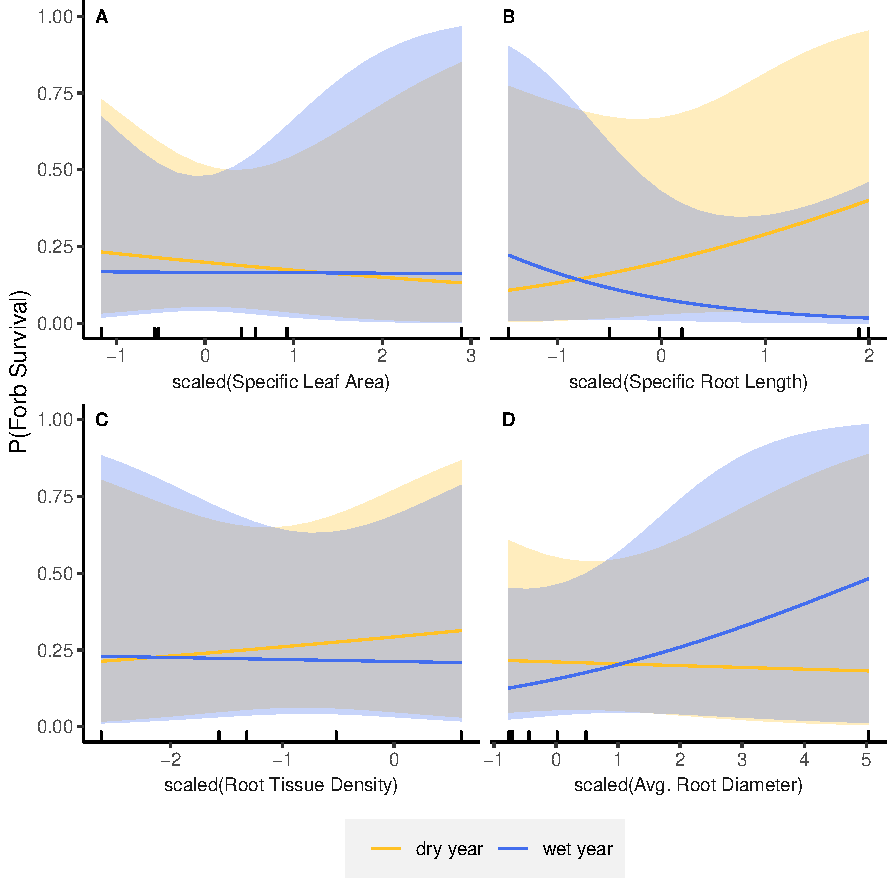
\includegraphics{figures/supForbSurvPlots-1.pdf}

Now make a figure showing model results for all growth models

\begin{Shaded}
\begin{Highlighting}[]
\CommentTok{\#get 2.5 and 97.5 percentiles of the distribution}
\NormalTok{meanSPEI \textless{}{-}}\StringTok{ }\KeywordTok{mean}\NormalTok{(CO\_grow\_TLP}\OperatorTok{$}\NormalTok{SPEI\_s)}
\NormalTok{sdSPEI \textless{}{-}}\StringTok{ }\KeywordTok{sd}\NormalTok{(CO\_grow\_TLP}\OperatorTok{$}\NormalTok{SPEI\_s)}
\CommentTok{\#get 97.5 quantile of the distribution}
\NormalTok{SPEI\_}\DecValTok{97}\NormalTok{\_}\DecValTok{5}\NormalTok{ \textless{}{-}}\StringTok{ }\KeywordTok{qnorm}\NormalTok{(.}\DecValTok{975}\NormalTok{, meanSPEI, sdSPEI) }
\NormalTok{SPEI\_}\DecValTok{2}\NormalTok{\_}\DecValTok{5}\NormalTok{ \textless{}{-}}\StringTok{ }\KeywordTok{qnorm}\NormalTok{(.}\DecValTok{025}\NormalTok{, meanSPEI, sdSPEI)}

\NormalTok{spei\_vals \textless{}{-}}\StringTok{ }\KeywordTok{c}\NormalTok{(SPEI\_}\DecValTok{2}\NormalTok{\_}\DecValTok{5}\NormalTok{, SPEI\_}\DecValTok{97}\NormalTok{\_}\DecValTok{5}\NormalTok{)}

\CommentTok{\#for TLP\_s}
\NormalTok{TLP\_vals \textless{}{-}}\StringTok{ }\KeywordTok{seq}\NormalTok{(}\KeywordTok{min}\NormalTok{(CO\_grow\_TLP}\OperatorTok{$}\NormalTok{TLP\_s, }\DataTypeTok{na.rm =} \OtherTok{TRUE}\NormalTok{), }\KeywordTok{max}\NormalTok{(CO\_grow\_TLP}\OperatorTok{$}\NormalTok{TLP\_s, }\DataTypeTok{na.rm =} \OtherTok{TRUE}\NormalTok{), }\DataTypeTok{length.out =} \DecValTok{20}\NormalTok{)}
\NormalTok{TLP\_grow\_dat \textless{}{-}}\StringTok{ }\KeywordTok{ggpredict}\NormalTok{(mGrowTLP, }\DataTypeTok{terms =} \KeywordTok{c}\NormalTok{(}\StringTok{"TLP\_s[TLP\_vals]"}\NormalTok{, }\StringTok{"SPEI\_s[spei\_vals]"}\NormalTok{), }\DataTypeTok{type =} \StringTok{"fixed"}\NormalTok{)}

\CommentTok{\#for LDMC\_s}
\NormalTok{LDMC\_vals \textless{}{-}}\StringTok{ }\KeywordTok{seq}\NormalTok{(}\KeywordTok{min}\NormalTok{(CO\_grow\_LDMC}\OperatorTok{$}\NormalTok{LDMC\_s, }\DataTypeTok{na.rm =} \OtherTok{TRUE}\NormalTok{), }\KeywordTok{max}\NormalTok{(CO\_grow\_LDMC}\OperatorTok{$}\NormalTok{LDMC\_s, }\DataTypeTok{na.rm =} \OtherTok{TRUE}\NormalTok{), }\DataTypeTok{length.out =} \DecValTok{20}\NormalTok{)}
\NormalTok{LDMC\_grow\_dat \textless{}{-}}\StringTok{ }\KeywordTok{ggpredict}\NormalTok{(mGrowLDMC, }\DataTypeTok{terms =} \KeywordTok{c}\NormalTok{(}\StringTok{"LDMC\_s[LDMC\_vals]"}\NormalTok{, }\StringTok{"SPEI\_s[spei\_vals]"}\NormalTok{), }\DataTypeTok{type =} \StringTok{"fixed"}\NormalTok{)}

\CommentTok{\#for RDMC\_s}
\NormalTok{RDMC\_vals \textless{}{-}}\StringTok{ }\KeywordTok{seq}\NormalTok{(}\KeywordTok{min}\NormalTok{(CO\_grow\_RDMC}\OperatorTok{$}\NormalTok{RDMC\_s, }\DataTypeTok{na.rm =} \OtherTok{TRUE}\NormalTok{), }\KeywordTok{max}\NormalTok{(CO\_grow\_RDMC}\OperatorTok{$}\NormalTok{RDMC\_s, }\DataTypeTok{na.rm =} \OtherTok{TRUE}\NormalTok{), }\DataTypeTok{length.out =} \DecValTok{20}\NormalTok{)}
\NormalTok{RDMC\_grow\_dat \textless{}{-}}\StringTok{ }\KeywordTok{ggpredict}\NormalTok{(mGrowRDMC, }\DataTypeTok{terms =} \KeywordTok{c}\NormalTok{(}\StringTok{"RDMC\_s[RDMC\_vals]"}\NormalTok{, }\StringTok{"SPEI\_s[spei\_vals]"}\NormalTok{), }\DataTypeTok{type =} \StringTok{"fixed"}\NormalTok{)}

\CommentTok{\#for SLA\_s}
\NormalTok{SLA\_vals \textless{}{-}}\StringTok{ }\KeywordTok{seq}\NormalTok{(}\KeywordTok{min}\NormalTok{(CO\_grow\_SLA}\OperatorTok{$}\NormalTok{SLA\_s, }\DataTypeTok{na.rm =} \OtherTok{TRUE}\NormalTok{), }\KeywordTok{max}\NormalTok{(CO\_grow\_SLA}\OperatorTok{$}\NormalTok{SLA\_s, }\DataTypeTok{na.rm =} \OtherTok{TRUE}\NormalTok{), }\DataTypeTok{length.out =} \DecValTok{20}\NormalTok{)}
\NormalTok{SLA\_grow\_dat \textless{}{-}}\StringTok{ }\KeywordTok{ggpredict}\NormalTok{(mGrowSLA, }\DataTypeTok{terms =} \KeywordTok{c}\NormalTok{(}\StringTok{"SLA\_s[SLA\_vals]"}\NormalTok{, }\StringTok{"SPEI\_s[spei\_vals]"}\NormalTok{), }\DataTypeTok{type =} \StringTok{"fixed"}\NormalTok{)}

\CommentTok{\#for RTD\_s}
\NormalTok{RTD\_vals \textless{}{-}}\StringTok{ }\KeywordTok{seq}\NormalTok{(}\KeywordTok{min}\NormalTok{(CO\_grow\_RTD}\OperatorTok{$}\NormalTok{RTD\_s, }\DataTypeTok{na.rm =} \OtherTok{TRUE}\NormalTok{), }\KeywordTok{max}\NormalTok{(CO\_grow\_RTD}\OperatorTok{$}\NormalTok{RTD\_s, }\DataTypeTok{na.rm =} \OtherTok{TRUE}\NormalTok{), }\DataTypeTok{length.out =} \DecValTok{20}\NormalTok{)}
\NormalTok{RTD\_grow\_dat \textless{}{-}}\StringTok{ }\KeywordTok{ggpredict}\NormalTok{(mGrowRTD, }\DataTypeTok{terms =} \KeywordTok{c}\NormalTok{(}\StringTok{"RTD\_s[RTD\_vals]"}\NormalTok{, }\StringTok{"SPEI\_s[spei\_vals]"}\NormalTok{), }\DataTypeTok{type =} \StringTok{"fixed"}\NormalTok{)}

\CommentTok{\#for SRL\_s}
\NormalTok{SRL\_vals \textless{}{-}}\StringTok{ }\KeywordTok{seq}\NormalTok{(}\KeywordTok{min}\NormalTok{(CO\_grow\_SRL}\OperatorTok{$}\NormalTok{SRL\_s, }\DataTypeTok{na.rm =} \OtherTok{TRUE}\NormalTok{), }\KeywordTok{max}\NormalTok{(CO\_grow\_SRL}\OperatorTok{$}\NormalTok{SRL\_s, }\DataTypeTok{na.rm =} \OtherTok{TRUE}\NormalTok{), }\DataTypeTok{length.out =} \DecValTok{20}\NormalTok{)}
\NormalTok{SRL\_grow\_dat \textless{}{-}}\StringTok{ }\KeywordTok{ggpredict}\NormalTok{(mGrowSRL, }\DataTypeTok{terms =} \KeywordTok{c}\NormalTok{(}\StringTok{"SRL\_s[SRL\_vals]"}\NormalTok{, }\StringTok{"SPEI\_s[spei\_vals]"}\NormalTok{), }\DataTypeTok{type =} \StringTok{"fixed"}\NormalTok{)}

\CommentTok{\#for RDiam\_s}
\NormalTok{RDiam\_vals \textless{}{-}}\StringTok{ }\KeywordTok{seq}\NormalTok{(}\KeywordTok{min}\NormalTok{(CO\_grow\_RDiam}\OperatorTok{$}\NormalTok{RDiam\_s, }\DataTypeTok{na.rm =} \OtherTok{TRUE}\NormalTok{), }\KeywordTok{max}\NormalTok{(CO\_grow\_RDiam}\OperatorTok{$}\NormalTok{RDiam\_s, }\DataTypeTok{na.rm =} \OtherTok{TRUE}\NormalTok{), }\DataTypeTok{length.out =} \DecValTok{20}\NormalTok{)}
\NormalTok{RDiam\_grow\_dat \textless{}{-}}\StringTok{ }\KeywordTok{ggpredict}\NormalTok{(mGrowRDiam, }\DataTypeTok{terms =} \KeywordTok{c}\NormalTok{(}\StringTok{"RDiam\_s[RDiam\_vals]"}\NormalTok{, }\StringTok{"SPEI\_s[spei\_vals]"}\NormalTok{), }\DataTypeTok{type =} \StringTok{"fixed"}\NormalTok{)}

\CommentTok{\#make a data.frame to contain all of the values for each trait}
\NormalTok{GrowthDat \textless{}{-}}\StringTok{ }\KeywordTok{data.frame}\NormalTok{(}\DataTypeTok{trait =} \KeywordTok{c}\NormalTok{(}\StringTok{"scaled(Turgor Loss Point)"}\NormalTok{), }\DataTypeTok{x =}\NormalTok{ TLP\_grow\_dat}\OperatorTok{$}\NormalTok{x, }\DataTypeTok{Growth =}\NormalTok{ TLP\_grow\_dat}\OperatorTok{$}\NormalTok{predicted, }\DataTypeTok{CI\_low =}\NormalTok{ TLP\_grow\_dat}\OperatorTok{$}\NormalTok{conf.low, }\DataTypeTok{CI\_high =}\NormalTok{ TLP\_grow\_dat}\OperatorTok{$}\NormalTok{conf.high, }\DataTypeTok{SPEI =}\NormalTok{ TLP\_grow\_dat}\OperatorTok{$}\NormalTok{group)}
\NormalTok{GrowthDat \textless{}{-}}\StringTok{ }\KeywordTok{rbind}\NormalTok{(GrowthDat, }\KeywordTok{data.frame}\NormalTok{(}\DataTypeTok{trait =} \KeywordTok{c}\NormalTok{(}\StringTok{"scaled(Leaf Dry Matter Content)"}\NormalTok{), }\DataTypeTok{x =}\NormalTok{ LDMC\_grow\_dat}\OperatorTok{$}\NormalTok{x, }\DataTypeTok{Growth =}\NormalTok{ LDMC\_grow\_dat}\OperatorTok{$}\NormalTok{predicted, }\DataTypeTok{CI\_low =}\NormalTok{ LDMC\_grow\_dat}\OperatorTok{$}\NormalTok{conf.low, }\DataTypeTok{CI\_high =}\NormalTok{ LDMC\_grow\_dat}\OperatorTok{$}\NormalTok{conf.high, }\DataTypeTok{SPEI =}\NormalTok{ LDMC\_grow\_dat}\OperatorTok{$}\NormalTok{group))}
\NormalTok{GrowthDat \textless{}{-}}\StringTok{ }\KeywordTok{rbind}\NormalTok{(GrowthDat, }\KeywordTok{data.frame}\NormalTok{(}\DataTypeTok{trait =} \KeywordTok{c}\NormalTok{(}\StringTok{"scaled(Root Dry Matter Content)"}\NormalTok{), }\DataTypeTok{x =}\NormalTok{ RDMC\_grow\_dat}\OperatorTok{$}\NormalTok{x, }\DataTypeTok{Growth =}\NormalTok{ RDMC\_grow\_dat}\OperatorTok{$}\NormalTok{predicted, }\DataTypeTok{CI\_low =}\NormalTok{ RDMC\_grow\_dat}\OperatorTok{$}\NormalTok{conf.low, }\DataTypeTok{CI\_high =}\NormalTok{ RDMC\_grow\_dat}\OperatorTok{$}\NormalTok{conf.high, }\DataTypeTok{SPEI =}\NormalTok{ RDMC\_grow\_dat}\OperatorTok{$}\NormalTok{group))}
\NormalTok{GrowthDat \textless{}{-}}\StringTok{ }\KeywordTok{rbind}\NormalTok{(GrowthDat, }\KeywordTok{data.frame}\NormalTok{(}\DataTypeTok{trait =} \KeywordTok{c}\NormalTok{(}\StringTok{"scaled(Specific Leaf Area)"}\NormalTok{), }\DataTypeTok{x =}\NormalTok{ SLA\_grow\_dat}\OperatorTok{$}\NormalTok{x, }\DataTypeTok{Growth =}\NormalTok{ SLA\_grow\_dat}\OperatorTok{$}\NormalTok{predicted, }\DataTypeTok{CI\_low =}\NormalTok{ SLA\_grow\_dat}\OperatorTok{$}\NormalTok{conf.low, }\DataTypeTok{CI\_high =}\NormalTok{ SLA\_grow\_dat}\OperatorTok{$}\NormalTok{conf.high, }\DataTypeTok{SPEI =}\NormalTok{ SLA\_grow\_dat}\OperatorTok{$}\NormalTok{group))}
\NormalTok{GrowthDat \textless{}{-}}\StringTok{ }\KeywordTok{rbind}\NormalTok{(GrowthDat, }\KeywordTok{data.frame}\NormalTok{(}\DataTypeTok{trait =} \KeywordTok{c}\NormalTok{(}\StringTok{"scaled(Specific Root Length)"}\NormalTok{), }\DataTypeTok{x =}\NormalTok{ SRL\_grow\_dat}\OperatorTok{$}\NormalTok{x, }\DataTypeTok{Growth =}\NormalTok{ SRL\_grow\_dat}\OperatorTok{$}\NormalTok{predicted, }\DataTypeTok{CI\_low =}\NormalTok{ SRL\_grow\_dat}\OperatorTok{$}\NormalTok{conf.low, }\DataTypeTok{CI\_high =}\NormalTok{ SRL\_grow\_dat}\OperatorTok{$}\NormalTok{conf.high, }\DataTypeTok{SPEI =}\NormalTok{ SRL\_grow\_dat}\OperatorTok{$}\NormalTok{group))}
\NormalTok{GrowthDat \textless{}{-}}\StringTok{ }\KeywordTok{rbind}\NormalTok{(GrowthDat, }\KeywordTok{data.frame}\NormalTok{(}\DataTypeTok{trait =} \KeywordTok{c}\NormalTok{(}\StringTok{"scaled(Root Tissue Density)"}\NormalTok{), }\DataTypeTok{x =}\NormalTok{ RTD\_grow\_dat}\OperatorTok{$}\NormalTok{x, }\DataTypeTok{Growth =}\NormalTok{ RTD\_grow\_dat}\OperatorTok{$}\NormalTok{predicted, }\DataTypeTok{CI\_low =}\NormalTok{ RTD\_grow\_dat}\OperatorTok{$}\NormalTok{conf.low, }\DataTypeTok{CI\_high =}\NormalTok{ RTD\_grow\_dat}\OperatorTok{$}\NormalTok{conf.high, }\DataTypeTok{SPEI =}\NormalTok{ RTD\_grow\_dat}\OperatorTok{$}\NormalTok{group))}
\NormalTok{GrowthDat \textless{}{-}}\StringTok{ }\KeywordTok{rbind}\NormalTok{(GrowthDat, }\KeywordTok{data.frame}\NormalTok{(}\DataTypeTok{trait =} \KeywordTok{c}\NormalTok{(}\StringTok{"scaled(Avg. Root Diameter)"}\NormalTok{), }\DataTypeTok{x =}\NormalTok{ RDiam\_grow\_dat}\OperatorTok{$}\NormalTok{x, }\DataTypeTok{Growth =}\NormalTok{ RDiam\_grow\_dat}\OperatorTok{$}\NormalTok{predicted, }\DataTypeTok{CI\_low =}\NormalTok{ RDiam\_grow\_dat}\OperatorTok{$}\NormalTok{conf.low, }\DataTypeTok{CI\_high =}\NormalTok{ RDiam\_grow\_dat}\OperatorTok{$}\NormalTok{conf.high, }\DataTypeTok{SPEI =}\NormalTok{ RDiam\_grow\_dat}\OperatorTok{$}\NormalTok{group))}

\CommentTok{\#make a data.frame with data for the rug plot}
\NormalTok{RugDat \textless{}{-}}\StringTok{ }\KeywordTok{data.frame}\NormalTok{(}\DataTypeTok{rug =}\NormalTok{ CO\_grow\_TLP}\OperatorTok{$}\NormalTok{TLP\_s, }\DataTypeTok{trait =} \StringTok{"scaled(Turgor Loss Point)"}\NormalTok{)}
\NormalTok{RugDat \textless{}{-}}\StringTok{ }\KeywordTok{rbind}\NormalTok{(RugDat, }\KeywordTok{data.frame}\NormalTok{(}\DataTypeTok{rug =}\NormalTok{ CO\_grow\_LDMC}\OperatorTok{$}\NormalTok{LDMC\_s, }\DataTypeTok{trait =} \StringTok{"scaled(Leaf Dry Matter Content)"}\NormalTok{))}
\NormalTok{RugDat \textless{}{-}}\StringTok{ }\KeywordTok{rbind}\NormalTok{(RugDat, }\KeywordTok{data.frame}\NormalTok{(}\DataTypeTok{rug =}\NormalTok{ CO\_grow\_RDMC}\OperatorTok{$}\NormalTok{RDMC\_s, }\DataTypeTok{trait =} \StringTok{"scaled(Root Dry Matter Content)"}\NormalTok{))}
\NormalTok{RugDat \textless{}{-}}\StringTok{ }\KeywordTok{rbind}\NormalTok{(RugDat, }\KeywordTok{data.frame}\NormalTok{(}\DataTypeTok{rug =}\NormalTok{ CO\_grow\_SLA}\OperatorTok{$}\NormalTok{SLA\_s, }\DataTypeTok{trait =} \StringTok{"scaled(Specific Leaf Area)"}\NormalTok{))}
\NormalTok{RugDat \textless{}{-}}\StringTok{ }\KeywordTok{rbind}\NormalTok{(RugDat, }\KeywordTok{data.frame}\NormalTok{(}\DataTypeTok{rug =}\NormalTok{ CO\_grow\_SRL}\OperatorTok{$}\NormalTok{SRL\_s, }\DataTypeTok{trait =} \StringTok{"scaled(Specific Root Length)"}\NormalTok{))}
\NormalTok{RugDat \textless{}{-}}\StringTok{ }\KeywordTok{rbind}\NormalTok{(RugDat, }\KeywordTok{data.frame}\NormalTok{(}\DataTypeTok{rug =}\NormalTok{ CO\_grow\_RTD}\OperatorTok{$}\NormalTok{RTD\_s, }\DataTypeTok{trait =} \StringTok{"scaled(Root Tissue Density)"}\NormalTok{))}
\NormalTok{RugDat \textless{}{-}}\StringTok{ }\KeywordTok{rbind}\NormalTok{(RugDat, }\KeywordTok{data.frame}\NormalTok{(}\DataTypeTok{rug =}\NormalTok{ CO\_grow\_RDiam}\OperatorTok{$}\NormalTok{RDiam\_s, }\DataTypeTok{trait =} \StringTok{"scaled(Avg. Root Diameter)"}\NormalTok{))}

\CommentTok{\#text for labels}
\NormalTok{dat\_text \textless{}{-}}\StringTok{ }\KeywordTok{data.frame}\NormalTok{(}
  \DataTypeTok{label =} \KeywordTok{c}\NormalTok{(}\StringTok{"A"}\NormalTok{, }\StringTok{"B"}\NormalTok{, }\StringTok{"C"}\NormalTok{, }\StringTok{"D"}\NormalTok{,}\StringTok{"E"}\NormalTok{,}\StringTok{"F"}\NormalTok{,}\StringTok{"G"}\NormalTok{),}
  \DataTypeTok{trait =} \KeywordTok{c}\NormalTok{(}\StringTok{"scaled(Turgor Loss Point)"}\NormalTok{, }\StringTok{"scaled(Leaf Dry Matter Content)"}\NormalTok{, }\StringTok{"scaled(Root Dry Matter Content)"}\NormalTok{, }\StringTok{"scaled(Specific Leaf Area)"}\NormalTok{, }\StringTok{"scaled(Specific Root Length)"}\NormalTok{, }\StringTok{"scaled(Root Tissue Density)"}\NormalTok{, }\StringTok{"scaled(Avg. Root Diameter)"}\NormalTok{),}
  \DataTypeTok{x    =} \KeywordTok{c}\NormalTok{(}\KeywordTok{min}\NormalTok{(TLP\_grow\_dat}\OperatorTok{$}\NormalTok{x), }\KeywordTok{min}\NormalTok{(LDMC\_grow\_dat}\OperatorTok{$}\NormalTok{x), }\KeywordTok{min}\NormalTok{(RDMC\_grow\_dat}\OperatorTok{$}\NormalTok{x), }\KeywordTok{min}\NormalTok{(SLA\_grow\_dat}\OperatorTok{$}\NormalTok{x),}\KeywordTok{min}\NormalTok{(SRL\_grow\_dat}\OperatorTok{$}\NormalTok{x),}\KeywordTok{min}\NormalTok{(RTD\_grow\_dat}\OperatorTok{$}\NormalTok{x),}\KeywordTok{min}\NormalTok{(RDiam\_grow\_dat}\OperatorTok{$}\NormalTok{x)),}
  \DataTypeTok{y     =} \KeywordTok{c}\NormalTok{(}\FloatTok{1.2}\NormalTok{,}\FloatTok{1.2}\NormalTok{,}\FloatTok{1.2}\NormalTok{,}\FloatTok{1.2}\NormalTok{,}\FloatTok{1.2}\NormalTok{,}\FloatTok{1.2}\NormalTok{,}\FloatTok{1.2}\NormalTok{)}
\NormalTok{)}

\CommentTok{\#make a multipanel figure}
\NormalTok{(GrowthExtraFig \textless{}{-}}\StringTok{ }\KeywordTok{ggplot}\NormalTok{(}\DataTypeTok{data =}\NormalTok{ GrowthDat) }\OperatorTok{+}
\StringTok{  }\KeywordTok{geom\_ribbon}\NormalTok{(}\KeywordTok{aes}\NormalTok{(}\DataTypeTok{x =}\NormalTok{ x, }\DataTypeTok{ymin =}\NormalTok{ CI\_low, }\DataTypeTok{ymax =}\NormalTok{ CI\_high, }\DataTypeTok{fill =}\NormalTok{ SPEI), }\DataTypeTok{alpha =} \FloatTok{0.3}\NormalTok{) }\OperatorTok{+}
\StringTok{  }\KeywordTok{geom\_line}\NormalTok{(}\KeywordTok{aes}\NormalTok{(}\DataTypeTok{x=}\NormalTok{x, Growth, }\DataTypeTok{col =}\NormalTok{ SPEI))  }\OperatorTok{+}\StringTok{ }
\StringTok{  }\KeywordTok{geom\_rug}\NormalTok{(}\KeywordTok{aes}\NormalTok{(}\DataTypeTok{x =}\NormalTok{ rug), }\DataTypeTok{data =}\NormalTok{ RugDat) }\OperatorTok{+}
\StringTok{  }\KeywordTok{labs}\NormalTok{(}\DataTypeTok{title =} \OtherTok{NULL}\NormalTok{) }\OperatorTok{+}
\StringTok{  }\KeywordTok{xlab}\NormalTok{(}\OtherTok{NULL}\NormalTok{) }\OperatorTok{+}
\StringTok{  }\KeywordTok{ylab}\NormalTok{(}\KeywordTok{expression}\NormalTok{(}\StringTok{"Graminoid Growth: log"} \OperatorTok{\textasciitilde{}}\StringTok{ }\KeywordTok{bgroup}\NormalTok{(}\StringTok{"("}\NormalTok{,}\KeywordTok{frac}\NormalTok{(size[year\_t}\OperatorTok{+}\DecValTok{1}\NormalTok{],size[year\_t]),}\StringTok{")"}\NormalTok{)))  }\OperatorTok{+}
\StringTok{  }\KeywordTok{scale\_color\_manual}\NormalTok{(}\DataTypeTok{labels =} \KeywordTok{c}\NormalTok{(}\StringTok{"dry year"}\NormalTok{, }\StringTok{"wet year"}\NormalTok{), }\DataTypeTok{values =} \KeywordTok{c}\NormalTok{(}\StringTok{"goldenrod1"}\NormalTok{, }\StringTok{"royalblue2"}\NormalTok{)) }\OperatorTok{+}
\StringTok{  }\KeywordTok{scale\_fill\_manual}\NormalTok{(}\DataTypeTok{values =} \KeywordTok{c}\NormalTok{(}\StringTok{"goldenrod1"}\NormalTok{, }\StringTok{"royalblue2"}\NormalTok{), }\DataTypeTok{guide =} \OtherTok{FALSE}\NormalTok{) }\OperatorTok{+}
\StringTok{  }\KeywordTok{facet\_wrap}\NormalTok{(}\KeywordTok{vars}\NormalTok{(trait), }\DataTypeTok{scales =} \StringTok{"free\_x"}\NormalTok{, }\DataTypeTok{strip.position =}  \StringTok{"bottom"}\NormalTok{) }\OperatorTok{+}
\StringTok{  }\KeywordTok{theme\_classic}\NormalTok{()}\OperatorTok{+}
\StringTok{  }\KeywordTok{theme}\NormalTok{(}\DataTypeTok{legend.position =} \StringTok{"bottom"}\NormalTok{, }\DataTypeTok{legend.title =} \KeywordTok{element\_blank}\NormalTok{(), }\DataTypeTok{legend.background =} \KeywordTok{element\_rect}\NormalTok{(}\DataTypeTok{fill=}\StringTok{"grey95"}\NormalTok{,}\DataTypeTok{size=}\FloatTok{0.5}\NormalTok{, }\DataTypeTok{linetype=}\StringTok{"solid"}\NormalTok{), }\DataTypeTok{strip.background =} \KeywordTok{element\_rect}\NormalTok{(}\DataTypeTok{colour=}\OtherTok{NA}\NormalTok{, }\DataTypeTok{fill=}\OtherTok{NA}\NormalTok{), }\DataTypeTok{strip.placement =} \StringTok{"outside"}\NormalTok{, }\DataTypeTok{strip.text.x =} \KeywordTok{element\_text}\NormalTok{(}\DataTypeTok{margin =} \KeywordTok{margin}\NormalTok{(}\DecValTok{0}\NormalTok{, }\DecValTok{0}\NormalTok{, }\FloatTok{1.5}\NormalTok{, }\DecValTok{0}\NormalTok{))) }\OperatorTok{+}
\StringTok{  }\KeywordTok{geom\_text}\NormalTok{(}\DataTypeTok{data=}\NormalTok{ dat\_text, }\DataTypeTok{mapping =} \KeywordTok{aes}\NormalTok{(}\DataTypeTok{x =}\NormalTok{ x, }\DataTypeTok{y =}\NormalTok{ y, }\DataTypeTok{label =}\NormalTok{ label), }\DataTypeTok{size =} \DecValTok{3}\NormalTok{, }\DataTypeTok{fontface =} \StringTok{"bold"}\NormalTok{))}
\end{Highlighting}
\end{Shaded}

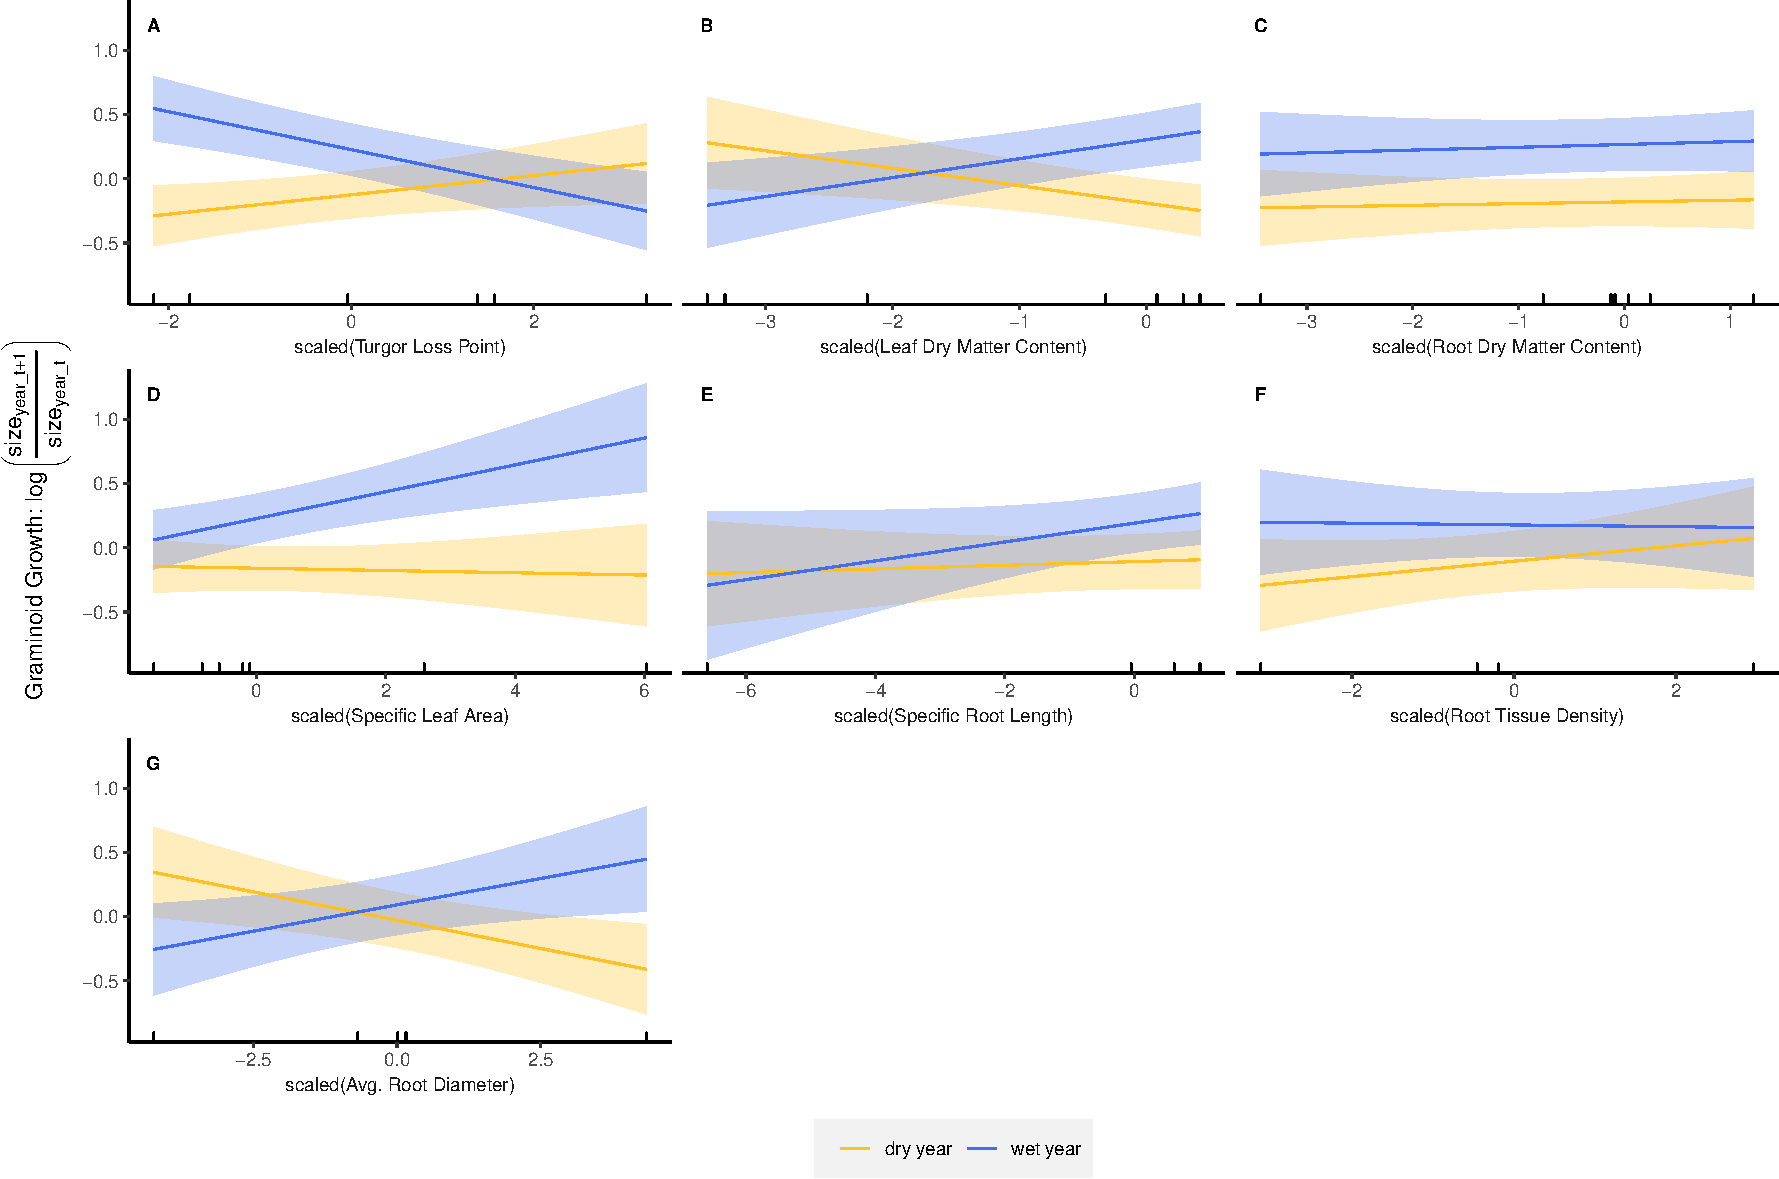
\includegraphics{figures/supGramGrowthPlots-1.pdf}

\end{document}
